%!TEX root = ../thesis.tex
%*******************************************************************************
%*********************************** Third Chapter *****************************
%*******************************************************************************

\chapter{Bioelectrical impedance plethysmography}  %Title of the First Chapter
\label{chapter impedance}

\ifpdf
    \graphicspath{{Chapter3/Figs/Raster/}{Chapter3/Figs/PDF/}{Chapter3/Figs/}}
\else
    \graphicspath{{Chapter3/Figs/Vector/}{Chapter3/Figs/}}
\fi

One of the primary objectives of this work is to produce a device capable of detecting, measuring, and quantifying changes in the venous and arterial circulation on a continuous basis. The most common method of measuring these changes is known as plethysmography. Armed with this information, it becomes possible to quantify changes in blood volume that can be translated into changes of blood volume or even flow rate.  Before delving deeper into the design of this device, it is necessary to understand the principles of operation and theories behind this technology. 

This chapter describes the underlying principles behind bioelectrical impedance plethysmography in greater detail. But before doing that, the effect of alternate current (AC) will be described to identify the safe limits when applied to the human body. Subsequently, the basics of the electrical impedance in conductors are illustrated, including the manner in which electrical current distributes in volumes. Next, the electrode-skin interface is examined in order comprehend how electric current conduction converts into ionic conduction. 

The bioelectrical impedance section elaborates on the effects of AC in the human body when interacting with cells and interpreting the data. A scope of the latest bioelectrical impedance technology will be described, which includes the essential components and methods needed to measure it. After explaining and understanding this basic premise, bioelectrical impedance plethysmography will be illustrated to demonstrate the key principles behind it and the signals that this kind of instrument are capable of producing are examined.  

\section{Electrical current in the human body} %Section - 3.7
\label{section impedance current in body}
Injecting electric current into biological tissue requires some safety measurements so as to guarantee the patients' welfare. Driving current into the human body may cause unpleasant effects such as heating, electrolysis at the electrode-tissue interface or neuromuscular stimulation \cite{martinsen2011bioimpedance, bertemes2002tissue}. The latter is the most dangerous negative effect because it controls thee element of blood circulation and respiration. Levels of current sensation vary from person-to-person, sex and are also predicated on the electrode geometry. However, Brown et al. \cite{brown1998medical} have established a threshold current whereby sensation increases when frequency rises, as shown in Figure \ref{fig:threshold sensation}. It has been recognised as the frequency dependency of the human body. The maximum sensitivity of the nervous system is in the frequency range between \SIrange[scientific-notation = engineering]{10}{1000}{\hertz}. At frequencies above \SI{1}{\kilo\hertz} sensitivity is considerably reduced and is entirely imperceptible above \SI{100}{\kilo\hertz}. In fact, the heat effect is so high at these frequencies that they can be used by electro-surgical devices. Square waves are not recommended because they combine the DC and AC effect in one signal wherein the duration of the pulse an important parameter to be controlled \cite{martinsen2011bioimpedance}.

\begin{figure}[!htpb]
	\centering
	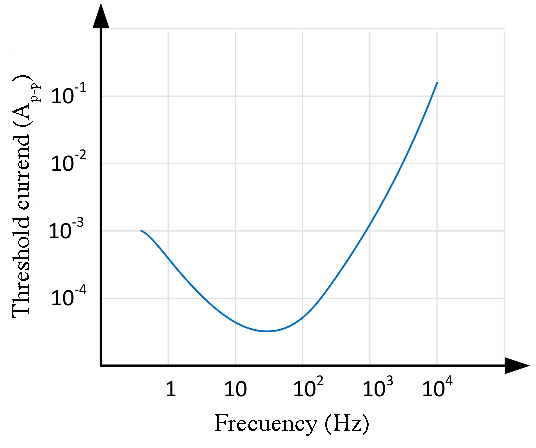
\includegraphics[width=0.45\textwidth,keepaspectratio]{figure14}    
	\caption[Threshold current sensation vs. frequency]{Threshold current sensation vs. frequency. Adapted from \cite{brown1998medical}}
	\label{fig:threshold sensation}
\end{figure}

The table \ref{table:current in body} illustrates the different levels of electric current tolerance of the human body. These effects are mostly predicated on current rather than frequency. When frequencies scale beyond \SI{100}{\kilo\hertz} especially on the radio-frequency (RF) range (\SIrange[scientific-notation = engineering]{400000}{3000000}{\hertz}) the heating effect of the tissue tends to be more common. As seen below, in order to avoid discomfort among patients, currents below \SI{5}{\milli\ampere} must be used in BIA device.

\begin{table}[!htpb]
	\caption{Effect of electric current in the human body}
	\centering
	\label{table:current in body}
	\begin{tabular}{lp{0.525\textwidth}}
		\toprule
		\textbf{Current Level}                &         \textbf{Effect}          \\ \midrule
		
		< \SI{1}{\milli\ampere}                &
		\begin{tabular}[t]{@{\textbullet~}p{0.5\textwidth}@{}} 
			Usually not perceptible 
		\end{tabular}
		\\\midrule
		\SI{1}{\milli\ampere}                  &
		\begin{tabular}[t]{@{\textbullet~}p{0.5\textwidth}@{}} 
			Threshold of current perception \\
			Tingling sensation
		\end{tabular}
		\\\midrule
		\SI{5}{\milli\ampere}                  &
		\begin{tabular}[t]{@{\textbullet~}p{0.5\textwidth}@{}} 
			Sensory nerve stimulation\\ 
			Shock sensation 
		\end{tabular}
		\\\midrule
		\SIrange{6}{25}{\milli\ampere} (Women) &
		\begin{tabular}[t]{@{\textbullet~}p{0.5\textwidth}@{}} 
			Painful electric shock \\ 
			Lack of muscular control 
		\end{tabular}
		\\\midrule
		\SIrange{9}{30}{\milli\ampere} (Men)   &
		\begin{tabular}[t]{@{\textbullet~}p{0.5\textwidth}@{}} 
			Difficult to let go - freezing current range \\
			High muscle contraction
		\end{tabular}	
		\\\midrule
		\SIrange{50}{150}{\milli\ampere}       &
		\begin{tabular}[t]{@{\textbullet~}p{0.5\textwidth}@{}} 
			Extreme pain \\
			Possible respiratory arrest \\
			Possible ventricular fibrillation (VF) \\
			Sever muscular contraction \\
			Possibly death
		\end{tabular}
		\\\midrule
		\SIrange{1}{4.3}{\ampere}              &
		\begin{tabular}[t]{@{\textbullet~}p{0.5\textwidth}@{}} 
			Heart's electric coordination compromised \\
			Muscular contraction and nerve damage \\
			Death likely 
		\end{tabular}
		\\\midrule
		\SI{10}{\ampere}                       &
		\begin{tabular}[t]{@{\textbullet~}p{0.5\textwidth}@{}} 
			Cardiac arrest \\
			Severe burns \\
			Highly probability of death
		\end{tabular}
		\\\bottomrule                            
	\end{tabular} 
\end{table}

Recommendations, guidelines and norms for patient safety are contained in international standards compiled by the International Electrotechnical Commission (IEC). The standard applicable to medical equipments or equipments to be used for humans is referenced as IEC 60601, or IEC 601. Some of these recommendations regarding safety are expressed as follows: first, the commission considers any frequency below \SI{0.1}{\hertz} as direct current in order to avoid ulcers created by electrode-skin interface; this type of current should be limited to \SI{10}{\uArms}. Moreover, for frequencies up to \SI{1}{\kilo\hertz}, it is recommended to limit the frequency of current at \SI{100}{\uArms}. Secondly, avoiding nerve stimulation is paramount for patient safety; at frequencies above \SI{1}{\kilo\hertz}, muscular stimulation becomes very difficult. Therefore, it is recommended to use frequencies higher than this value. Thirdly, one important recommendation of the standard is that the maximum amount of current flowing through skin contact must be limited to \SI{0.5}{\milli\ampere} with a single fault equipment \rvmynote{I have to check this, becuase it rises questions}. Lastly, as explained before, in the RF range tissue that could be heated, tissue burns can be avoided by limiting the density and duration of current; for instance, it is recommended to use densities of less than \SI{1}{\milli\ampere\per\milli\meter\squared}. In terms of practical applications of current vs. frequency, for frequencies above \SI{1}{\kilo\hertz}, the Commission has established the equation \ref{eq:current body} to calculate the maximum root-mean-square current when this is less than \SI{10}{\mArms}.

\begin{align}
	\label{eq:current body}
	I_{MAX(RMS)} = 10^{-7}.f
\end{align}

where $f$ is the frequency of the measurement.

\section{Electrical impedance principle}
\label{section impedance principle}
%https://books.google.co.uk/books?id=M74ecVj5q9UC&printsec=frontcover&dq=inauthor:%22Luca+Callegaro%22&hl=en&sa=X&ved=0ahUKEwjMyPSt5MnSAhUJJcAKHZAPBGcQ6AEIHDAA#v=onepage&q&f=false
From the electrical point standpoint, impedance is defined as the opposition that a medium presents to either an alternating current (AC) or voltage (see figure \ref{fig:impedance}) \cite{callegaro2012electrical}. Impedance is equal to the complex ratio between electrical voltage and current. This mathematical fraction produces a complex number which is known as symbol $Z$ (see equation \ref{eq:Z magnitude}). This comprises of a resistance (also known as conductance) and/or reactance value, which is commonly represented by the letters $R$ and $X$ respectively. Hence, the impedance measurement can be expressed as a relation of the output magnitude and the phase difference between real and imaginary parts, as shown in equation \ref{eq:phasor}; it can be plotted in the complex plane as shown in figure \ref{fig:complex impedance}.

\begin{figure*}[!htpb]
	\centering
	\begin{subfigure}[t]{0.4\textwidth}
		\centering
		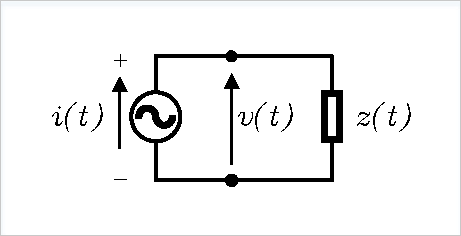
\includegraphics[width=6cm,trim={0.05cm 0.05cm 0.05cm 0.15cm},clip,keepaspectratio]{figure0a}    
		\caption{Current driven impedance}
		\label{fig:impedance a}
	\end{subfigure}
	~
	\begin{subfigure}[t]{0.4\textwidth}
		\centering
		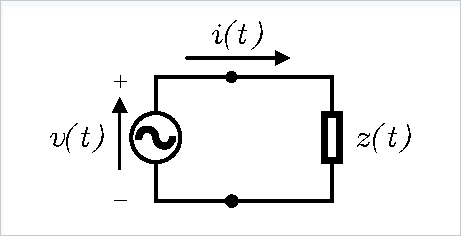
\includegraphics[width=6cm,trim={0.05cm 0.05cm 0.05cm 0.15cm},clip,keepaspectratio]{figure0b}    
		\caption{Voltage driven impedance}
		\label{fig:impedance b}
	\end{subfigure}
	\caption[Impedance representation from two-terminal element]{Schematic of the electrical impedance. The three elements that are required are the voltage $v(t)$, the alternating current $i(t)$ and the opposition to the current ($z(t)$). The impedance can be driven by either current or voltage.}
	\label{fig:impedance}
\end{figure*}

\begin{align}
	\label{eq:phasor}
	Z = \lvert Z \rvert  \angle \phi
\end{align}

There are different ways to represent impedance. However, bioelectrical impedance can be described in the form of either resistance ($R$) or reactance ($X$). Notaby, in this complex number, the resistive part signifies the real actual part of the measurement, whereas the reactance constitutes an imaginary one. Therefore, the impedance magnitude can be written as a function in these two values, as illustrated in the equation \ref{eq:Z magnitude}.

\begin{figure}[!htpb]
	\centering
	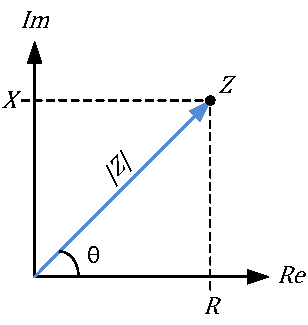
\includegraphics{figure_2}    
	\caption[Complex representation of impedance]{Plot of the impedance in the complex plane.}
	\label{fig:complex impedance}
\end{figure}

\begin{gather}
	\label{eq:Z magnitude}
	Z = Z' + Z'' = R + jX = \lvert Z \rvert e^{j\theta}\\
	|Z| = \sqrt{Z Z^{*}} = \sqrt{R^2 + X^2} \\
	\theta = tan^{-1}\frac{X}{R} \\
	\label{eq:resistance}
	R = \lvert Z \rvert cos(\theta) \\
	\label{eq:reactance}
	X = \lvert Z \rvert sin(\theta)
\end{gather}

As seen above, when the angle difference of the impedance is \SI{0}{\degree}, the load is completely resistive. In contrast, when the phase difference is \SI{90}{\degree} the load is purely reactive. On the basis of the previous equations, it is possible to represent impedance in the complex plane, as illustrated in figure \ref{fig:complex impedance}.

Another way to express and analyse impedance is using sinusoidals. For instance, when a sinusoidal steady-state waveform injects a current $i(t) = I_A cos(\omega t)$ into an unknown load, the response is a shifted in a sinusoidal waveform with a potential equivalent of $v(t) = V_B cos(\omega t + \phi)$. Figure \ref{fig:impedance wave} illustrates the representation of both waveforms. Hence, the impedance can be denoted as the ration of these two quantities based on Ohm's law (see equation \ref{eq:ohm}).

\begin{align}
	\label{eq:ohm}
	Z = \frac{V}{I}
\end{align}

\begin{figure}[!htpb]
	\centering
	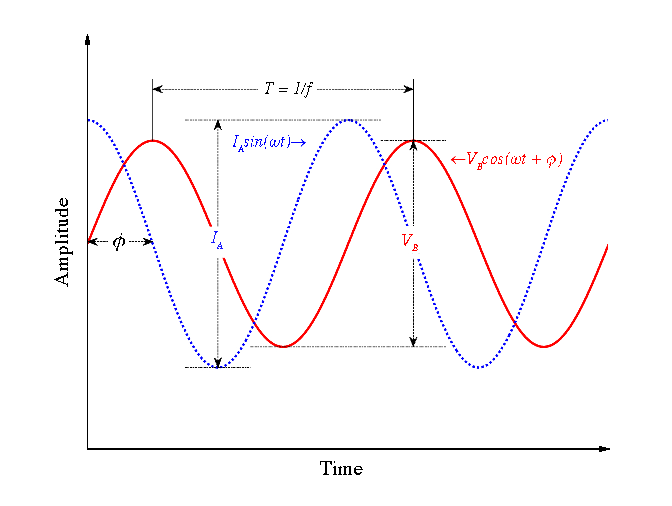
\includegraphics[width=0.8\textwidth,keepaspectratio, trim={0cm 0cm 0cm 0cm},clip]{figure_1}    
	\caption[Impedance waveforms]{Waveform plot of a current ($I_A cos (\omega t)$) compared to the potential representation ($V_B cos (\omega t + \phi)$) of an unknown load.}
	\label{fig:impedance wave}
\end{figure}


However, performing mathematical operations with trigonometry identities could be quite tedious. Therefore, equivalent methods are used in order to analyse impedance in an electric circuit. Using Euler's formula allows us to express trigonometric functions in order of $e$. The equation \ref{eq:euler} illustrates the relation between both entities.

\begin{equation}
\label{eq:euler}
e^{j\omega t} = cos(\omega t) + j sin(\omega t)
\end{equation}  

Therefore, voltage and current can be rewritten in the form of complex exponential thanks to Euler's equation. 

\begin{align}
	\label{eq:volatge euler}
	v(t) = V_B cos(\omega t + \phi) = V_B(e^{j(\omega t + \phi)}) \\
	\label{eq:current euler}
	i(t) = I_A cos(\omega t) = I_A(e^{j\omega t})	
\end{align}

Using Ohm equation \ref{eq:ohm} makes it possible to calculate the resultant impedance of the waveforms. Therefore, the expression using complex exponentials would be equal to:

\begin{align}
	\label{eq:complex Z}
	Z = \frac{v(t)}{i(t)} = \frac{V_B(e^{j(\omega t + \phi)})}{I_A(e^{j\omega t})} = \frac{V_B}{I_A} e^{j\phi}
\end{align}

Based on Euler's equation, it is possible deduct the real and imaginary parts of the complex exponential of equation \ref{eq:complex Z}.

\begin{align}
	\label{eq:complex Z2}
	Z = \frac{V_B}{I_A} e^{j\phi} = \frac{V_B}{I_A}(cos(\phi) + j sin(\phi)
\end{align}

Using the principle of superposition, it becomes possible to assume that the real and imaginary components of impedance are signified by the following formulae that are equivalents to the ones obtained with phasor analysis equations	\ref{eq:resistance} and \ref{eq:reactance}.

\begin{align}
	\label{eq:R Z}
	Z' = R = \frac{v(t)}{i(t)} = \frac{V_B}{I_A}cos(\phi) \\
	\label{eq:X Z}
	Z'' = X = \frac{v(t)}{i(t)} = \frac{V_B}{I_A}sin(\phi)
\end{align}

In conclusion, it is possible to obtain real and imaginaries values of impedance if the maximum amplitude of the voltage ($V_B$) and current ($I_A$) are known, in addition to their difference in phase ($\phi$). 

\section{Current distribution in conductors (Geselowitz theorem)}  %Section - 3.4
\label{section impedance Geselowitz}
Geselowitz \cite{geselowitz1971application} studied the change in conductivity within a constant geometry. In short, his analysis entailed the application of lead field theory into electrical impedance. Simplifying the origin of the equation, the total impedance of the entire volume is equivalent to the sum of all the small impedances within each small volume $dV$ \cite{martinsen2011bioimpedance}.

\begin{figure}[!htpb]
	\centering
	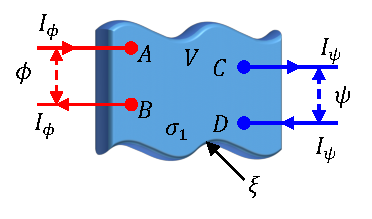
\includegraphics[width=6.3cm,keepaspectratio]{figure9}    
	\caption[Volume conductor with 4 electrodes]{Volume conductor $V$ of conductivity $\sigma_1$. A:B represent current injection electrodes and C:D are sensing electrodes.}
	\label{fig:volume}
\end{figure}

The analysis of this equation begins from the study of the four-electrode measurement and the change in conductivity of the internal region of a volume conductor \cite{bertemes2002tissue}. Figure \ref{fig:volume} posits that a volume conductor is electrically linear and surrounded by an insulator $\xi$. If the internal conductivity changes from $\sigma_1$ to $\sigma_2$ (equivalent to $\sigma_1+\Delta \sigma$) then the potential field of the current injection will change from $\phi$ to $\phi \prime$ (equal to $\phi+\Delta \phi$) although the potential field $\psi$ will remain unchanged. Then, the field equation will be as follows:

\begin{align}
	\label{eq:potential field}
	\int_{\Omega} \sigma . (\phi - \phi \prime) . \nabla \psi d \overline{S} = \int_{V} (\sigma_1 - \sigma_2).(\nabla \phi \prime \bullet \nabla \psi).dV 
\end{align}

By replacing the terms with the equivalents, the equation can be rewritten in accordance to the next equation.

\begin{align}
	\label{eq:potential field2}
	- \Delta \phi_{CD} . (-I_{\psi}) = - \int_{V} \Delta \sigma . [\nabla (\phi + \Delta \phi) \bullet \nabla \psi].dV
\end{align}

The impedance change can be deducted by dividing the function by the currents involved $I_{phi}$ and $I_{\psi}$. As a result, the Geselowitz equation is equivalent to:

\begin{align}
	\label{eq:Geselowitz}
	\Delta Z = \frac{\Delta \phi_{CD}}{I_\phi} = - \int_V \Delta \sigma (x,y,z).\bigg[\frac{\nabla(\phi + \Delta \phi)}{I_{\phi}} \bullet \frac{\nabla \psi}{I_{\psi}}\bigg].dV
\end{align}

The previous equation is the key to calculating the change in impedance in a volume within defined boundaries. However, this only applies to homogeneous and isotropic volume conductors. The equation can be simplified if is assumed that a unit of current passes through and the volume conductor can be denoted by a number of discrete elements of uniform conductivity within a three dimensional space ($x,y,z$). As a result, the equitation can be simplified as follows:

\begin{align}
	\label{eq:Geselowitz2}
	\Delta Z = - \Delta \sigma \cdot \int_V \nabla(\phi + \Delta \phi) \bullet \nabla \psi . dV = - \Delta \sigma \cdot S
\end{align}

where $S$ denotes the sensitivity matrix in three dimensions; it is independent of conductance. Calculating this variable requires a series of assumptions, such as the initial conductivity distribution being uniform \cite{dehghani1999incorporating}. This document is not centred on the mathematical analysis of the sensitivity $S$, but deducting those impedance changes are directly related to the change of geometry within this segment. Several studies provide credence to the fact that sensitivity varies in accordance to the electrodes position and geometry, as researched by Filho \cite{bertemes2002tissue}.

\section{Electrode-skin interface}  %Section - 3.3
\label{section impedance electrodes}
Electrodes play a key role in a bioelectrical impedance system. The nuances of electrode geometry, distance and material may influence the readings from a biological standpoint. Consequently, electrodes with minor impedance are required to be used, as opposed to the one from the subject under test. Currently, most common materials used in bioelectrical impedance include platinum (\textit{Pt}), gold (\textit{Au}) or stainless steel. Other independent variables such temperature, ionic tissue contents and protein adhesion also influence the changes of electrode impedance~\cite{martinsen2011bioimpedance, ivorra2003bioimpedance}. The geometry of the electrode also affects its resistance ($R$) as explained by Ohm's law in this equation: \ref{eq:resist}.

\begin{align}
	\label{eq:resist}
	R = \rho \frac{L}{A}
\end{align}

where $\rho$ denotes the electrical resistivity of the material, $A$ refers to the area of the electrode, and $L$ signifies the longitude or thickness. The resistance ($R$) reduces when the area ($A$) of the electrode increases. However, the total resistance ($R$) is directly proportional to the length of electrodes. 

When an electrode adheres to the skin and electrical current passes through, a physical effect takes place. To begin with, an electrical charge change occurs from electronic to ionic conduction because only the latter is possible inside the body. Second, at the electrode-tissue boundary, an electrochemical reaction follows, known as electrolysis. This effect creates a "double layer capacitance (DLC)" (see figure \ref{fig:DLC}) which, as its name indicates, adds a capacitive effect to boundary \cite{lvovich2012impedance}. Consequently, applying an AC waveform inverts the electrode polarity during each cycle, thereby minimising this capacitive effect. However, this is a frequency dependent development, implying it can be quite notorious that at low frequencies \cite{bertemes2002tissue}.  

\begin{figure}[!htpb]
	\centering
	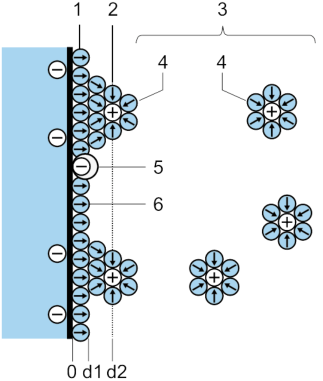
\includegraphics[width=5.5cm,keepaspectratio]{figure7}    
	\caption[Dual layer representation on an electrode]{Schematic representation of a double layer on an electrode (BMD) model. 1. Inner Helmholtz plane, (IHP), 2. Outer Helmholtz plane (OHP), 3. Diffuse layer, 4. Solvated ions (cations) 5. Specifically, adsorbed ions (redox ion, which contributes to the phase shift element). Image from \cite{lvovich2012impedance}}
	\label{fig:DLC}
\end{figure}

An electric circuit model can denote the electric-tissue interface; this simplified electric representation is shown in figure \ref{fig:e-t circuit}. This model is characterised by a charge transfer resistance ($R_{CT}$) in parallel with the interface's impedance ($Z_{CPE}$) in congruity with the tissue impedance ($Z_t$).  Some authors have defined the interface's impedance as either a constant phase or angle impedance ($Z_{CPA}$) \cite{franks2005impedance} or constant phase element ($C_{PE}$) \cite{barsoukov2005impedance, mcadams2006characterization}. 

\begin{figure}[!htpb]
	\centering
	\begin{circuitikz}
		\draw[american](0,0) 
		to[short, n=met] (2,0)
		to[short, o-*] (2,0) -- (2,1)
		to[generic=$Z_{CPE}$] (4,1) -- (4,0)
		to[short, o-*] (4,0)
		to[generic=$Z_t$, n=res] (6,0)
		(2,0) -- (2,-1)
		to[R=$R_{CT}$](4,-1)--(4,0)
		
		(met.s) node[below]{Metal}
		(res.s) node[below]{Tissue}
		;
	\end{circuitikz}   
	\caption[Equivalent circuit electrode-tissue interface]{Equivalent circuit electrode-tissue interface (Adapted from Franks~\cite{franks2005impedance})}
	\label{fig:e-t circuit}
\end{figure}

The value of $Z_{ZPA}$ can be calculated from the following empirical equation: \ref{eq:zcpa} given by McAdams~\cite{mcadams1995linear}.

\begin{align}
	\label{eq:zcpa}
	Z_{CPA} = K(j\omega)^{-\beta}
\end{align}

where $K$ denots a measure of the magnitude of $Z_{CPA}$, $\beta$ represents a constant ($0 \leq \beta \leq 1$) signifying inhomogeneities in the surface (typically \num{0.8} for a number of biomedical electrode systems) and $\omega = 2\pi f$. When $\beta = 1$, $Z_{CPE}$ is equivalent to a purely capacitive impedance element \cite{franks2005impedance,mcadams2006characterization,mcadams1995linear}.

Electrodes are also a source of error when taking measurements. Some blunders can even distort the original signal; for instance, thermal noise is also known as Johnson-Nyquist noise. This type of noise is entirely inherent to the electrode and is predicated on external variables.  The equation \ref{eq:nyquist noise} represents the level of noise attributed to the electrode~\cite{mcadams1995linear}.

\begin{align}
	\label{eq:nyquist noise}
	V_n(rms)=\sqrt{(4 K_b T R \Delta f)}
\end{align}

where $K_b$ is Boltzmann constant, $T$ denotes absolute temperature, $R$ signifies the electrode resistance, and $\Delta f$ denotes the bandwidth of the measurements. 

In summation, noise ($V_n(rms)$) can be considered directly proportional to the bandwidth measurements ($\Delta f$). At high operating frequency is expected to result in a higher the level of noise. In the case of impedance plethysmography, the bandwidth lies in the lower range of \si{\kilo\hertz} to minimise the effect of the Johnson-Nyquist noise.

Another source of errors caused by electrode can be derived from their position in the body, lack of surface contact, or mismatch in materials and geometries. Therefore, in order to improve and maximise the area of contact, some electrodes necessitate conductive gel. Using commercially available electrodes for electrocardiogram (ECG) purposes has been proven to provide good impedimetric readings, as opposed to specially designed electrodes~\cite{caicedo2012use}.

An experiment using this type of electrodes was conducted to determine whether removing one or four electrodes and putting them back in the same position could cause errors in readings. It was found that putting electrodes away and then getting them back into the same position for an extended period caused minimum changes in impedance readings. Most of the changes were presented in terms of the variations in the geometry of the body segment (being tested) were caused by the electrodes reposition that might have varied either through the current path or the voltage reading. One of the most important conclusions was that a suitable way of mitigating the effect of electrode repositioning ,the measurement should be to calculate the impedance ratio at different frequencies~\cite{lozano1997electrode}.

At the moment of taking measurements for localised bioelectrical impedance using tetrapolar configuration, the distribution of the electrodes does impact the sensitivity of the system along with the geometry of the cells contained within the tissue ~\cite{bertemes2002tissue}. According to experiments, the separation of injection and detection electrode pairs affects the existing depth of penetration. In other words, the bigger the separation between the pair of electrodes, the deeper the AC signal are likely to go.


\section{Bioelectrical impedance}
\label{section impedance BI}
Before describing the manner in which impedance plethysmography operates, it would be more prudent to understand how the principle of bioelectrical impedance is defined. Firstly, the term electrical impedance spectroscopy (EIS) refers to the study of the absorption of energy in accordance to the frequency of electromagnetic (EM) waves. When measurements are performed in a biological sample, this method could be referred to as either electrical bioimpedance or bioelectrical impedance~\cite{ivorra2003bioimpedance}. The term to be used in the context of this document will be bioelectrical electrical impedance. Given that the EM spectrum is quite broad, and the interaction with tissue occurs in the frequency range from \SIrange[scientific-notation = engineering]{100}{10000000}{\hertz}~\cite{bertemes2002tissue}. In this thesis, the frequencies of interest are focused in a low spectrum range. Indeed, plethysmography devices are known to commonly operate in the radio wave frequency of the electromagnetic spectrum.

The human body comprises of four basic tissues known as epithelium, muscle, connective tissue and nervous tissue. Epithelium covers the whole surface of the body. On the other hand, muscles are in charge of the movement, whereas connective tissues impart protection to organs. Nervous tissue provides the internal transmission line for the electrical impulses coming from the brain. Cells that create these tissues play a fundamental role with regard to current conduction when an analogue current (AC) is applied to the body~\cite{lvovich2012impedance}. Hence, impedance readings vary based on the parameters of these cells and their protein content. It is especially important to understand the geometry and characteristics of the blood cells, which transport $0_2$ around the body. The functionality of these cells and amount per \si{\micro\litre} of human blood have been described by Table \ref{table:cell} in section \ref{section literature circulatory system}.

As shown in the table, there are RBCs than any other cells, and they entail particular resistive properties. Its disk shape can be ideally represented as a spherical particle with membranes around the surface, as represented by Figure \ref{fig:cell}. Live cells can be represented as multilayer cells where its internal cytoplasm has a specific permittivity ($\epsilon_{cp}$) and conductivity ($\rho_{cp}$). Likewise, these characteristics are similar to the one surrounding the cell known as extracellular fluid ($\epsilon_m$ and $\rho_m$). However, the membrane suffers from a very low permittivity ($\epsilon_{MBR}$) and conductivity ($\rho_{MBR}$) behaving as a dielectric. In contrast, the membrane becomes loose in the case of dead cells and does not provide resistance to electric current~\cite{lvovich2012impedance}.

\begin{figure}[!htpb]
	\centering
	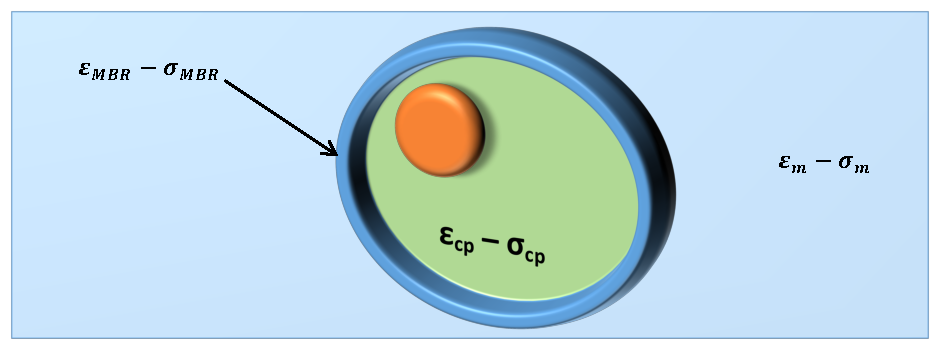
\includegraphics[width=0.8\textwidth,keepaspectratio, trim={0cm 0cm 0cm 0cm},clip]{figure1}    
	\caption[Cell permeability and conductivity distribution]{Representation of a cell with its electric characteristics. Internal cytoplasm characteristic permittivity $\epsilon_{cp}$ and conductivity $\rho_{cp}$. Extracellular fluid permittivity $\epsilon_m$ and conductivity $\rho_m$). Membrane permittivity described as ($\epsilon_{MBR}$) and conductivity ($\rho_{MBR}$).}
	\label{fig:cell}
\end{figure}

A cell can change its internal cytoplasm using two different means, either changing the permeability of their bilayer lipid membrane (BLM) or through the use of ionic channels or pumps. The BLM is about \SI{7}{\nano\meter} thick. Altering its permeability allows lipids and water molecules to pass through~\cite{ivorra2003bioimpedance}. The interface between the extracellular space, the cell membrane and intracellular space ($\rho_m \rightarrow \rho_{MBR} \leftarrow \rho_{cp}$) behave as a capacitor since membrane is a dielectric between two conductors, denoted as $C_m$ in figure \ref{fig:cell model}.

In contrast, parallel to BLM, the ionic channels and pumps enhance the functionality of membranes. Ionic channels or "channel proteins" allow for the transport and exchange of certain types of ions such as $Na^{+}$, $K^{+}$, Chloride ($Cl^{-}$) and Calcium ($Ca^{2+}$) between the inside and outside part of the cell~\cite{lvovich2012impedance}. Ion pumps are caused by sensitivity of the membrane to a voltage and are responsible for the membrane's non-linear properties as a response to low voltage. This pump causes cell polarisation, enabling the flow of ion charges in the body. Electrically, these channels act as a resistor ($R_m$).

\begin{figure*}[!htbp]
	\centering
	\begin{subfigure}[t]{0.48\textwidth}
		\centering
		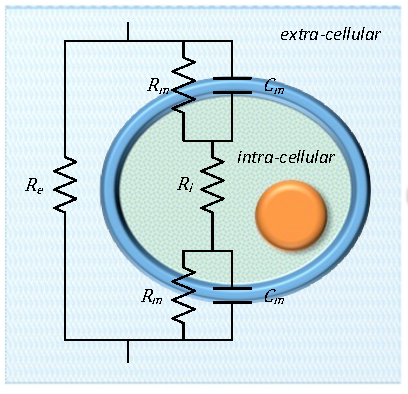
\includegraphics[height=6.5cm]{figure2a}
		\caption{Cell's equivalent circuit model}
		\label{fig:cell model}
	\end{subfigure}%
	~ 
	\begin{subfigure}[t]{0.48\textwidth}
		\centering
		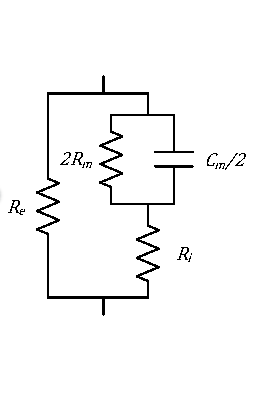
\includegraphics[height=6.5cm]{figure2b}
		\caption{Simplified circuit model}
		\label{fig:cell simp model}
	\end{subfigure}
	\caption[Electrical model of the cell]{Electrical model of the cell and its simplified version. $R_e$ is the resistivity of the extracellular medium, $R_i$ is the resistivity of the intracellular medium and $R_m$ and $C_m$ are the resistivity and capacitance of the membrane.}
	\label{fig:cell models}
\end{figure*}

According to previous analysis, the cell can be simplified in an equivalent electric circuit model, as shown in Figure \ref{fig:cell models}. This model indicates that if AC is pumped into the extracellular medium, there are two possible paths for the current to go through. One way is around the cell - represented by the resistive characteristic of the extracellular medium ($R_e$). Under the second route, current flows through the cell. It is possible that AC flows initially either over the BLM, which is represented as a capacitance ($C_m$), or across ionic channels ($R_m$). Upon reaching the cell, current travels via the intracellular medium ($R_i$) that is mostly resistive. Finally, the electrical current exits from the cell through the membrane, which again lies in the same $C_m$ and $R_m$.

Since $C_m$ and $R_m$ share the same values when the current enters and exits the cell, this can be simplified in the electric model as the two resistors in series ($2R_m$) and two capacitances are parallel to each other ($C_m/2$) as indicated by figure \ref{fig:cell simp model}.

When an EM field is applied on the tissue, cells respond based on the frequency applied, highlighting three distinctive areas in the spectrum, as described by Schwan et al.~\cite{schwan1957electrical,schwan1962electrical}. Figure \ref{fig:ABG dispersion} displays the dielectric response against frequency, which reveals valuable information about the functional and structural properties of the cell~\cite{lvovich2012impedance}. According to the graph, there are three denominating areas $\alpha$, $\beta$ and $\gamma$ dispersion. Firstly, $\alpha$ dispersion (from \SI{10}{\hertz} to a few \si{\kilo\hertz}) is generally associated with frequency dependent properties of the cells' membrane. Secondly, $\beta$ dispersion (\SI{10}{\kilo\hertz} to several \si{\mega\hertz}) is related to the dielectric property of the cell membrane as well as the interaction between the internal and external mediums. Finally, $\gamma$ dispersion (> \SI{10}{\giga\hertz}) is attributed to the dielectric relaxation of bulk dispersing media, the Debye dispersion in water (\SI{17}{\giga\hertz}), and the presence of small molecules. 

\begin{figure}[!htpb]
	\centering
	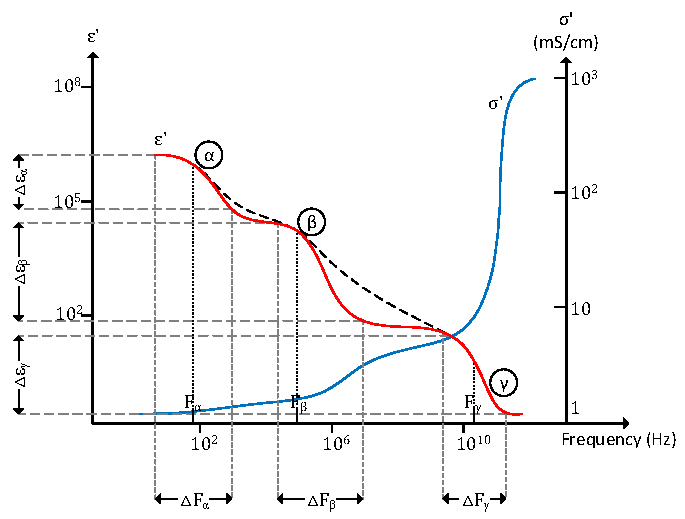
\includegraphics[width=0.8\textwidth,keepaspectratio, trim={0cm 1cm 0cm 0cm},clip]{figure3}    
	\caption[Alpha, Bet y Gama dispersion]{Representation of a cell with its electric characteristics. Internal cytoplasm characteristic permittivity $\epsilon_{cp}$ and conductivity $\rho_{cp}$. Extracellular fluid permittivity $\epsilon_m$ and conductivity $\rho_m$). Membrane permittivity described as ($\epsilon_{MBR}$) and conductivity ($\rho_{MBR}$).}
	\label{fig:ABG dispersion}
\end{figure}

In addition, the $\beta$ dispersion region provides supplementary information about the cell. Lvovich \cite{lvovich2012impedance} divides this area into three subregions in accordance to the interaction of the electrical current with the cell. The $\beta_1$ relaxation is caused by the capacitive membrane $C_m$, occurring in the low \si{\kilo\hertz} range. When the frequency increases between \si{\kilo\hertz} and low \si{\mega\hertz} range, the internal cytoplasm of the cell produces a $\beta_3$ dispersion owning to a change from resistive to capacitive conduction. However, this capacitive component is often disregarded, thereby simplifying the model into a resistive element $R_i$. Ultimately, $\beta_2$ occurs in the range of low \si{\mega\hertz} when the electrical charge movement through the cell shifts into a capacitive conduction.

This research document is centred on the $\beta$ dispersion region between \SIrange[scientific-notation = engineering]{100}{1000000}{\hertz}. The impedance plethysmography device designed described in chapter \ref{chapter design} can operate in a diverse range of programmable frequencies up to \SI{100}{\kHz}. 

The ideal electrical model of the cell is shown in figure \ref{fig:cell models} is a very close approximation that facilitates the prediction of bioelectrical impedance behaviour for dilute cell suspension. However, the tissue is more complex than this particular simplified model because it is comprised of additional elements that must be added to the analysis. For instance, tissues like muscle exhibits extreme anisotropy (conductivity is not the same when measured in different directions) \cite{lvovich2012impedance,dean2008electrical,foster1995dielectric}. In addition, different resistivity values have been obtained when measuring bioelectrical impedance during the cardiac cycle longitudinally and transversely \cite{steendijk1993four}. Another instance of how impedance changes in the context of tissues properties can be seen in the performed by Casas et al. \cite{casas1999vivo}. This study showed the differences between normal and ischemic tissue of a pig's myocardium muscle. Impedance clearly presented a different impedimetric response when a frequency sweep was done between \SIrange[scientific-notation = engineering]{10}{1000000}{\hertz}. 

\subsection{Mathematical representation of electrical impedance}
Electrical impedance can yield a different response based on the frequency. In a bioelectrical impedance analysis (BIA), the impedimetric response needs to be represented as a function of the frequencies used along with the magnitude and phase obtained. Different mathematical models have been studied based on the basic and ideal framework, as shown in figure \ref{fig:cell simp model}. However, this model does not entirely encapsulate the effect of the membrane at high frequencies. Debye came up with the following equation that took the suspension of free poles into consideration \cite{bertemes2002tissue}.

\begin{align}
	\label{eq:Debye}
	\varepsilon_r^* = \varepsilon_{HF} + \frac{\varepsilon_{LF} - \varepsilon_{HF}}{1 + j \omega \tau}
\end{align}

In this equation, $\varepsilon_r^*$ signifies the complex relative permeability, $\varepsilon_{LF}$ and $\varepsilon_{HF}$ represents the permeability at low and high frequency, respectively and $\tau$ denotes the relaxation time constant. Meanwhile $j \omega =2 \pi$ refers to the angular frequency in radians. However, it was not until 1941 when Cole brothers took into account, dispersion by factoring the Debye equation that an additional parameter called $\alpha$ resulted in the equation \ref{eq:cole cole}. This mathematical formula is widely used to obtain the approximate value of impedance during the course of taking biomedical measurements \cite{cole1941dispersion}.

\begin{align}
	\label{eq:cole cole}
	\varepsilon_r^* = \varepsilon_{HF} + \frac{\varepsilon_{LF} - \varepsilon_{HF}}{(1 + j \omega \tau)^{1-\alpha}}
\end{align}

The parameter $\alpha$ is limited for values between 0 and 1. When its value is equal to zero, the Cole-Cole equation will yield the Debye equation (\ref{eq:Debye}) as a solution for polar dielectrics. Consequently, from this mathematical statement, it is possible to obtain data representation known as the Cole-Cole plot. It is a two-dimensional graph where the plot of $\varepsilon \prime\prime$ or the imaginary part of the equation lies in the $y$-axis vs $\varepsilon \prime$ in the $x$-axis, which forms the real part of the solution. 

The representation of data using Cole-Cole representation allows to see changes in frequency for different tissues. This information is valid when spectroscopy studies are being performed. Regarding the most suitable frequency to measure impedance plethysmography, whole body bioelectrical impedance analysis has shown that limbs contributed significantly to the impedance at frequencies \SIlist{0.5; 50; 100}{\kHz} \cite{bracco1996segmental}. Therefore, any AC with this frequency spectrum is suitable for an impedance plethysmography instrument. 

\section{Bioelectrical impedance state of the art} %Section - 3.5
\label{section impedance state art}
Either a bioimpedance device or impedance plethysmography device operates under the principles described before. However, there are different alternatives to circuits and methods to measure impedance from the human body.  

Currently, no efforts are being made to implement impedance into wearable technologies. For instance, Samsung Electronics has released a hand-wrist size wearable device called simband~\cite{simsense}. In their product announcement, Samsung uses electrical impedance in order to measure the galvanic impedance response (GSR) and Bio-Impedance (Bio-Z). In figure \ref{fig:simsense} the actual sensor band (simsense) is exhibited in its second generation counts with different sensors in addition to the ones previously mentioned. These include electrocardiogram signals (ECG), photoplethysmography (PPG), accelerometers and skin temperature. Nevertheless, this kind of device falls into the research spectrum and continues to be under development.

\begin{figure}[!htpb]
	\centering
	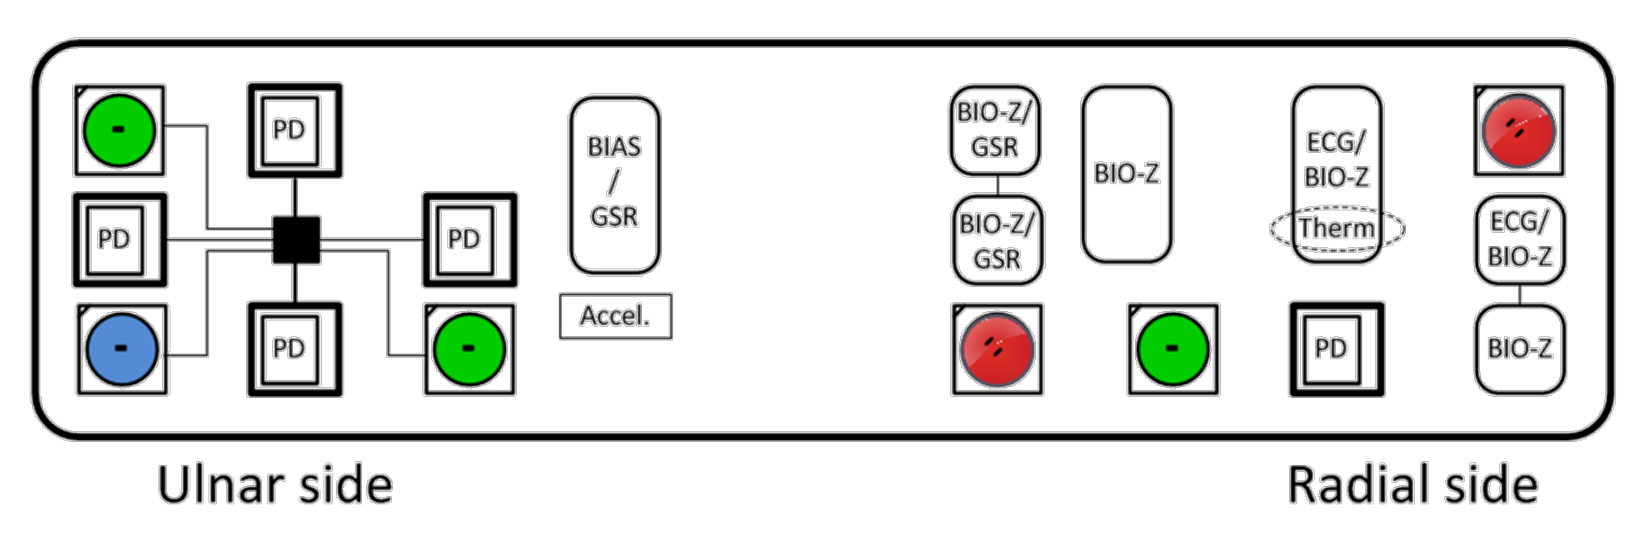
\includegraphics[width=8cm,keepaspectratio]{figure10}    
	\caption[\nth{2} generation Simsense board for the Simband]{\nth{2} generation Simsense board for the Simband. Image from \cite{simsense}}
	\label{fig:simsense}
\end{figure}

However, a significant number of devices use bioimpedance for different medical applications, such as impedance cardiography (ICG) devices. They have been developed to measure different properties of the heart such as stroke volume (SV), cardiac output (CO) and systemic vascular resistance (SVR)~\cite{neath2005utility}.  Nevertheless, apart from its main application, this instrument has also been used to measure other medical parameters such as proximal vein thrombosis (PVT)~\cite{hull1978impedance} or the levels of ischemia during orthopaedic surgery~\cite{distefano1973bioelectrical}.

Some companies are also working towards creating alternative medical applications for bioelectrical impedance technology. One example of this is the Australian company ImpediMed~\cite{impedimed} which owns the patents for this technology and has manufactured FDA-approved commercial devices focused on detecting body fluid contents in three areas: Lymphedema product line designed to detect lymphatic obstruction conducting in the context of inflammation and liquid retention.  Fluid Status/Body Composition product line is intended to measure water and fat content in the human body. BMI research product is another of its product designed to calculate body mass index (BMI) using bioelectrical impedance analysis.

Another company that has successfully created a FDA approved medical device using bioelectrical impedance in the market is Cheetah Medical \cite{cheetah} from Israel. This company based out of Boston (US) has quire remarkably, developed a product to gauge the haemodynamics non-invasive using as many as four electrodes configuration. The device is used in different hospital areas such as critical care, haemodialysis, emergency department and operating theatres.

Tanita Corporation, a Japanese company that has emerged as a pioneer in the field of digital weight scales, has come up with a device capable of performing a whole body composition analysis using bioelectrical spectroscopy analysis or segmental bioelectrical impedance methods~\cite{tanita}. These FDA approved products can accomdoate an enormous number of readings from the human body, including extracellular water content (EWC), intracellular water content (IWC), muscle balance, segmental analysis of muscle mass and fat percentage.

Finally, German company medis (Medizinische Messtechnik GmbH) \cite{medis} is a spin-off company from Institute of Biomedical Engineering of the Technical University Ilmenau. They manufacture medical equipment for the purpose of cardiovascular diagnosis, including impedance cardiograph and impedance plethysmography devices. However, their devices are combined with other methods such as PPG and ECG to obtain a better assessment of the haemodynamics. 

\section{Basic components of a bioelectrical impedance device}
\label{section impedance basic}
Evidently, there are several medical that incorporate either biomedical or bioelectrical impedance technology. Nonetheless, regardless of the application, most of the instruments include in their design, the block diagram illustrated in figure \ref{fig:block diagram bioimpedance} within their designs. 

\begin{figure}[!htpb]
	\centering
	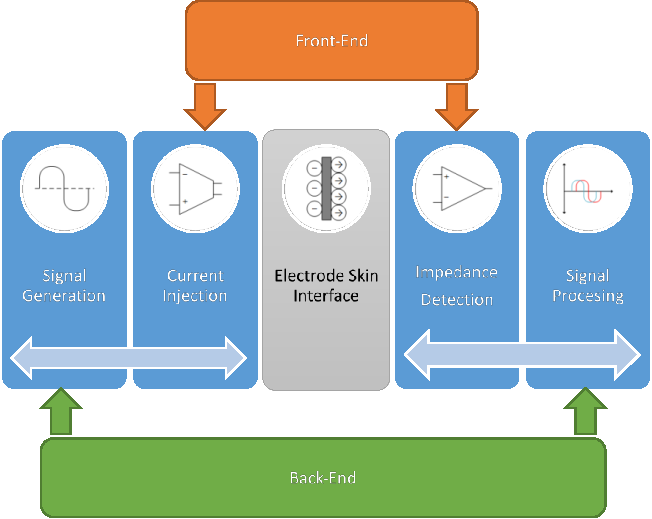
\includegraphics[width=9cm,keepaspectratio]{figure11}    
	\caption[Block diagram of a common bioimpedance device]{An bioimpedance device requires front-end and back-end components in order to detect changes of impedance efficiently.}
	\label{fig:block diagram bioimpedance}
\end{figure}

An impedance system can be categorized into three different blocks: the first one known as back-end commonly comprises of signal generation and digital analysis circuits in order to evaluate the sensed signal. Next is the front-end block comprised of all the circuitry before establishing contact with the skin, such as current injection and signal detection electronics. Ultimately, skin electrode interface behaving as an electronic circuit has been described in section \ref{section impedance electrodes}. 

Meanwhile the back-end block is divided into two different sections. First signal generation circuits depend on either extremely precise oscillators or Digital Signal Synthesizers (DDS) to generate accurate signal waves in a wide bandwidth with highly accurate amplitudes. The frequency exactness of these electronic circuits could scale up to \SI{0.1}{\percent} \cite{ad:AD5930}.  Different kind of waveforms may be applied, but a sinusoidal wave is the most common one. 

Signal processing circuits lie at the other end of the spectrum, and are used to evaluate a signal's amplitude and phase sensed by the front-end block.  Notably, powerful processors or microprocessors are used to analyse and digitise the signals identified. Moreover, modern devices are also aided by either Digital Signal Processors (DSP) or high-speed analogue to digital converters (ADC) that are capable of oversampling the detected signals. This level of precision in high-speed processors and chips makes them highly specialised and expensive.

Likewise, the front-end is divided into two different sections: current injection and signal detection circuits. The current injection circuit, as indicated by its name, transmits the signal coming from the wave generator into the electrodes; some characteristics of these circuits are high bandwidth, accuracy and linearity. 

On the other hand, signal detection circuits receive the signal after having passed through the sample under test. As opposed to specialised digital circuitry used on the back-end, the front-end mostly relies on highly precise analogue systems. These circuits can be implemented with discrete components or custom chips. However, discrete components may evince a limited response when there is a requirement of bandwidths in the order of Megahertz. Consequently, custom microchip design replete with current injection and sensing circuits are a better option because it reduces the influence of stray capacitances. 

\subsection{Methods of measuring bioelectrical impedance}
\label{section impedance state art.1}
Some authors have utilised the bioelectrical impedance analysis (BIA) the method to interpret impedance measurements from the human body \cite{kyle2004bioelectrical}. Different techniques have been developed using a single/multiple frequencies or varying amounts of electrodes. This section describes the most common type of BIA techniques; it explains their operation frequency, electrodes location, and data representation.

\subsubsection{Single Frequency BIA}
Single frequency bioimpedance analysis uses a single frequency to perform the whole body impedance analysis. The most common frequency used for this purpose is \SI{50}{\kilo\hertz}, primarily used for body composition analysis where current is made to flow through the entire body by applying electrodes on the hands and feet in a tetrapolar set-up, as displayed in Figure \ref{fig:single f BIA}. This method can provide an insightful approach to whole body composition analysis, including free-fat mass (FFM) and a weighted sum of ECW and ICW resistivities \cite{kyle2004bioelectrical}. Nonetheless, the measurements can be significantly affected by the subject's hydration level \cite{gudivaka1999single,schoeller2000bioelectrical}.

\begin{figure}[!htpb]
	\centering
	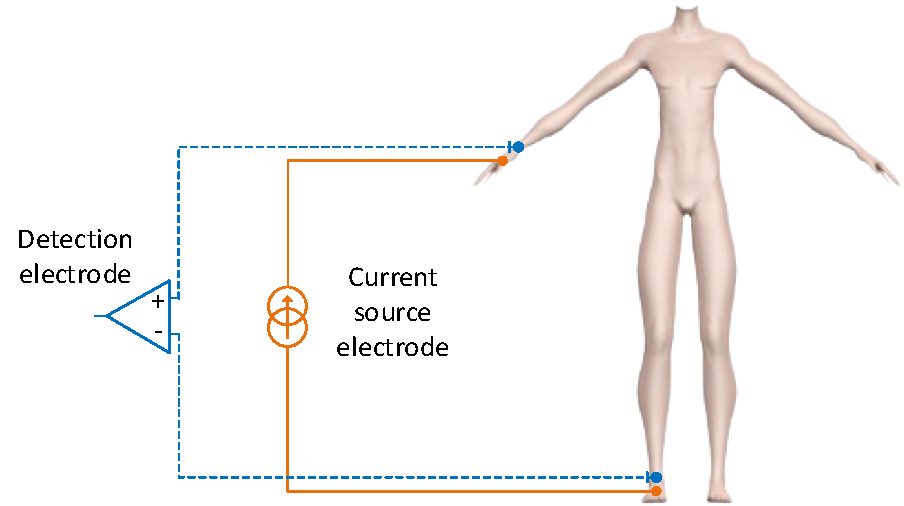
\includegraphics[width=0.7\textwidth,keepaspectratio]{figure12}    
	\caption[Common electrodes placement for whole body BIA and BIS]{Common electrode location for single frequency BIA, multi-frequency BIA and BIS (Adapted from Kyle \cite{kyle2004bioelectrical})}
	\label{fig:single f BIA}
\end{figure}

\subsubsection{Multi-frequency BIA}
This method is very similar to the one described previously; it also focuses on the whole body analysis. However, this technique uses empirical linear regression models and multiple set frequencies to evaluate total body water (TBW), FFM, ICW and ECW. Likewise, it has been shown to be an effective tool to assess amyotrophic lateral sclerosis (ALS) \cite{wang2011electrical}. The most common frequencies used in this regard are \SIlist{1;5;50;100;200;500}{\kilo\hertz} \cite{kyle2004bioelectrical}. 

However, some studies have revealed that there is a poor reproducibility in frequencies below \SI{5}{\kilo\hertz} and above \SI{200}{\kilo\hertz}. Also, multi-frequency BIA has recorded some improvements as compared to single frequency BIA when measuring similar parameters in the body; however, their clinical significance is inadequate \cite{hannan1995comparison}. LSTLY, single frequency BIA has been observed to be more accurate in calculating TBW in critically ill subjects, whereas multi-frequency BIA is more accurate and less biased in predicting ECW \cite{patel1996estimation}. 

\subsubsection{Bioelectrical impedance spectroscopy (BIS)}
Although multi-frequency BIA and BIS entail the incorporation of a broad range of frequencies, BIS uses mathematical analysis and a mixture of equations to find the whole body equivalent impedance. One of these mathematical analysis' is the implementation of the Cole-Cole \cite{cole1941dispersion} calculation, as shown in Equation \ref{eq:cole cole} and mixing theory model from Hanai \cite{hanai1968electrical}. These models make it possible to provide additional information about TBW and ECW \cite{hanai1968electrical}. 

For this method to work effectively it needs to be able to use mathematical models, constants and equations obtained from a healthy population \cite{patel1994estimation}. If this technique needs to be utilised for a specific purpose or population, such as monitoring a disease, there is a need to apply either a new calibration or a different mathematical model so as to get a more accurate correlation between the predictions and the results \cite{schoeller2000bioelectrical, de1997predicting}. However, using a combination of different methods has shown different results, some of them being accurate, with others showing no improvement or even worse results as compared to previous techniques using regression approaches \cite{kyle2004bioelectrical}. The use of BIS can be made more accurate if previous data is known to fit the better curve in relation to the results. As a result, some researchers have implemented the use of neural networks in order to predict the results according to previous readings \cite{songer2001tissue,kun2003algorithm}. 

\subsubsection{Segmental bioelectrical impedance analysis}
This method requires applying two additional electrodes in other parts of the body, such as opposite wrist and foot, wrist and shoulder, upper iliac spine and ankle, proximal part of the forearm and lower leg, as well as shoulder and upper thigh. However, there is no standardisation in the position of these electrodes, which might lead to different current distribution for whole body measurements \cite{kyle2004bioelectrical, woodrow1996segmental}. A good correlation has been observed between appendicular lean body mass evaluated by X-ray absorptiometry (DXA) and segmental BIA adjusted by stature at all frequencies. Moreover, upper extremities constitute the main component of impedance at high frequencies (order of \si{\kHz}) because there is generally a higher fat content in arms than in legs \cite{delorenzo2003segmental}. 

However, this method has not been recommended in healthy young adults due to the possibility of inaccuracy \cite{laforgia2008body,leahy2012comparison}. Calculating TBW requires measuring the length of body segments (arm, trunk and leg) in order to make calculations for the analysis, but Thomas et al. \cite{thomas2003comparison} opine that this extra effort is not justified when similar outputs can be obtained with BIA method. In contrast, segmental BIA has been found useful in calculating fluid distribution in some illnesses like ascites (abnormal accumulation fluid in the abdominal cavity) and during surgery \cite{kyle2004bioelectrical}. Moreover, it has been found to be very practical for patients with renal failure, where the imbalance of fluids can be detected more accurately \cite{woodrow1996segmental,thomas2003comparison}. 

\subsubsection{Localised bioelectrical impedance analysis}
All the previous methods have focused on whole body measurements. On the other hand, localised BIA aims to avoid the incidence of the effects of different variables, such as hydration, fat fraction, geometry boundary conditions, etc. Focusing on well-defined segments of the body enables the minimisation of the effect of these variables. Moreover, when the segment is confined to a small volume, it becomes possible to calculate plethysmography or blood flow. The use of four electrodes assumes great significance for such applications because it creates the boundaries of such a system. 

The calculation of BIA also simplifies because it facilities the application of empirical regression models as per their populaiton\cite{kyle2004bioelectrical}. Some cases involve the dimensions of the limb being studied in order to obtain its geometric volume for a more detailed calculation.  Some cases where this technique has been successfully applied include the analysis of limb ischemia \cite{songer2001tissue, kun1994tissue} breast cancer \cite{zou2003review}, detection and monitoring of Lymphedema \cite{vicini2012bioelectrical} and local abdominal fat mass \cite{scharfetter2001assessing}. 

\subsubsection{Bioelectrical impedance vector analysis}
This method was developed by Piccoli et al. \cite{piccoli2000relationship, piccoli2002impedance} at the beginning of 2000 to asses fluid body volume through uncovering patterns of vector distribution based on resistance ($R$) and admittance ($X_{c}$) values \cite{thomas2003comparison}. On top of those values, BIVA requires height and genre from the patient so as to establish a statistical ranking as compared to similar population (reference population). 

\begin{figure}[!htpb]
	\centering
	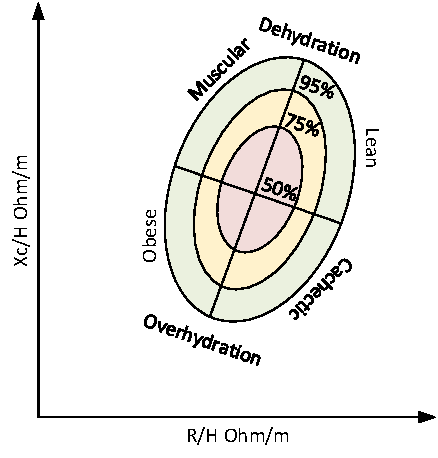
\includegraphics[width=0.4\textwidth,keepaspectratio]{figure13}    
	\caption[BIVA representation]{BIVA representing the vector distribution based on resistance and admittance}
	\label{fig:BIVA plot}
\end{figure}

Data is represented in a graph $R$ vs. $X_{c}$, which compares the subject's data to ellipses tolerances from the reference population at \SIlist{50;75;95}{\hertz} that was previously calculated in a healthy population of the same race, the age and sex \cite{kyle2004bioelectrical,piccoli2000relationship, piccoli2002impedance}. As an illustration, if a measurement falls below \SI{75}{\percent} on the left of right of the ellipse, it can indicate an anomaly in tissue's impedance. This data can be interpreted as changes in tissue hydration and varying amounts of body cell mass (BCM) in a lean body tissue. BIVA has been validated for different medical instances for the management of body hydration such as in acute heart failure, haemodialysis, hydration, diuresis, ultrafiltration and body hydration in emergency room \cite{disomma2011consensus}. 

\section{The principle of bioelectrical impedance plethysmography} 
\label{section iPG principle}
As previously described in section \ref{section literature BI}, iPG denotes the measurement of volume changes through the equivalent impedance of a human body part \cite{corciova2011peripheral}. Indeed, when heart's systole increases the blood flow, the volume of a limb rises due to the inflow of arterial blood (swelling) \cite{martinsen2011bioimpedance}. Consequently, there are changes of impedance that are correlated to the changes of volume as well as flow in any part of the body. Some of the medical applications of this technology include the measurement of heart stroke volume (SV), cardiac output (CO), thoracic respiratory volume, oedema as well as the detection of deep vein thrombosis (DVT)~\cite{holohan1996plethysmography}.  

The genesis of impedance plethysmography can be traced back to the model that was proposed by Jan Nyboer~\cite{nyober1950electrical}. The author describes extremities as cylinders, where in an inner cylinder signifies a blood vessel, and surrounding tissue accounts for the outermost part. The whole electrical conductance path results from the sum of the parallel conductance of blood and tissue within a segment. In fact, this theory known as parallel conductor was subsequently confirmed by the experiments performed by Shimazu et al. \cite{shimazu1982evaluation}. There have been some doubts about the extent of the blood's impedance contribution to the total impedance signal. Nonetheless, the in-vitro experiment demonstratd that blood (haematocrit = $ 26 \pm 4 \%$) contributed to \SI{10}{\percent} of the impedance signal. In the study, the final result was obtained when comparing the measurements of a saline buffer solution and blood in extensible arteries as well as rigid tubes~\cite{peura1978influence}.

\begin{figure}[!htpb]
	\centering
	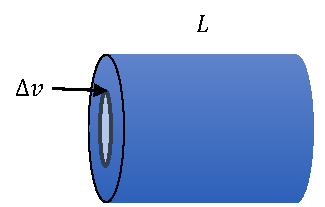
\includegraphics[width=5.5cm,keepaspectratio]{figure5}    
	\caption[Two compartment cylinder model]{Two compartment cylinder model of length L and parallel volume increment}
	\label{fig:two cylinder model}
\end{figure} 

In principle, recurring to the anatomy that was described in the section \ref{section literature anatomy}, the normal volume ($V$) of a human forearm contain within a certain length $L$, the bones, muscle, fat and blood structure around a cross-sectional area ($A$) (see figure \ref{fig:two cylinder model}). When a circulatory cycle takes place, an additional amount of blood enters the limb through the brachial artery to raise total volume of the limb in $\Delta V$. Thus, the new limb's total volume at the peak of this systole will be equivalent to $V + \Delta V$. As a result, shunting impedance $Z_b$ is produced by the following equation \cite{swanson1976origin, webster2009medical}:

\begin{align}
	\label{eq:blood impedance}
	Z_b = \rho_b \frac{L}{\Delta A}
\end{align}

where $\rho_b$ denotes the blood's conductivity and $\Delta A$ refers to the increase of in the cross-sectional area of the limb. However, for this formula to work, some assumptions need to be taken into consideration: the arterial expansion is uniform along the tissue, the blood resistivity ($\rho$) remains constant, and the flow of current is parallel to the artery \cite{bera2014bioelectrical}. Therefore, the artery volume change can be obtained by using the following formula \cite{swanson1976origin, webster2009medical}.

\begin{align}
	\label{eq:delta volume}
	\Delta V = L \times \Delta A = \rho_b \frac{L^2}{\Delta A}
\end{align}

During the cardiac cycle, the area of the artery increases from $A$ to $A + \Delta A$. However, the impedance of $Z_b$ is also affected by the additional impedance ($\Delta Z$) that is produced by the increment $\Delta A$, and this $Z_b$ is connected in parallel to $Z$. Therefore, Nyboer \cite{nyober1950electrical} postulated that the practical parallel resistive value of the displaced blood can originate from the parallel relation between the initial base resistance and the new resistance value, signified by the following expression:

\begin{align}
	\label{eq:parallel model}
	\Delta Z = (Z_b \parallel Z) - Z = \frac{Z^2}{Z + Z_b}
\end{align}

where $Z$ is equivalent to the limb's original resistance at diastole and $Z_b$ represents the increase of new total resistance. $Z_b \gg Z$, then $Z_b$ can now be rewritten as:

\begin{align}
	\label{eq:parallel model2}
	\frac{1}{Z_b}\cong -\frac{\Delta Z}{Z^2}
\end{align}

Finally, the changes in limb volume in association with the variation of impedance are denoted by the equation \ref{eq:nyober dV}. It must be noted that the negative sign is an indication of direction.

\begin{align}
	\label{eq:nyober dV}
	\Delta V = -\rho_b \frac{L^2}{Z^2}\Delta Z
\end{align}

Different equations are derived by complementing Nyboer's work. One of the modifications is the Kubicek et al. method~\cite{karnegis1966development, kubicek1970impedance, kubicek1979impedance}. His equation is widely used, especially when taking the measurements of impedance cardiography from the thoracic box and deducting stroke volume of the heart. Another popular work is the contribution  of Sramek~\cite{sramek1986bomed}. The author also modified Kubicek's equation by eliminating the dependence $L$ and $\rho_b$,  and introduced a constant that was obtained using statistical methods named "volume of electrical participating tissue". Alternative calculation methods have been developed using admittance instead of impedance.

In his research and patent work, Yamakoshi \cite{yamakoshi1980limb, shimazu1982evaluation, yamakoshi1978admittance} uses impedance reciprocate and admittance $(Y=Z^{-1})$ to estimate blood flow using plethysmography which performed better with analogue computers of the time. In his work, the author states that the first gradient of the computation result to time indicates the blood rate in the limb being examined. However, the algorithms used in this study will be confined to the equations proposed by Nyboer.

\subsection{Two or four electrode measurements}
\label{section iPG electrodes}
Various electrode topologies are used to take impedance measurements. Some of these options include two-electrode, three electrode and four electrode setting. The following analysis describes the difference between the two most common options: bipolar and tetrapolar electrodes.

As described in section \ref{section impedance electrodes}, the circuit model of an electrode is equivalent to a charge transfer resistance ($R_{CT}$) in parallel to an unknown interface impedance ($Z_{CPE}$); these two components represent the impedance and polarization of the electrode-electrolyte interface \cite{neuman2000biomedical} in congruity with a the tissue impedance ($Z_t$) \cite{lvovich2012impedance}. Completing this model also requires the inclusion of half-cell potential, which is denoted as a battery ($E_{hc}$) \cite{neuman2000biomedical}. Therefore, the complete electrode model can be modelled as shown in figure \ref{fig:electrode model}.

\begin{figure}[!htpb]
	\centering
	\begin{circuitikz}
		\draw[american](0,0) 
		to[battery=$E_{hc}$] (2,0)
		to[short, o-*] (2,0) -- (2,1)
		to[generic=$Z_{CPE}$] (4,1) -- (4,0)
		to[short, o-*] (4,0)
		to[generic=$Z_t$] (6,0)
		(2,0) -- (2,-1)
		to[R=$R_{CT}$](4,-1)--(4,0)
		;
	\end{circuitikz}
	\caption[Electrode equivalent circuit]{The electrical model of an electrode is equivalent to a battery representing the half-cell potential, }
	\label{fig:electrode model}
\end{figure}

The most common option to measure impedance within the body is the tetrapolar option. The following analysis illustrates the ideal cases when using two and four electrodes in the measurements.

\subsubsection{Bipolar electrode measurement}
The bipolar electrodes method uses the same pair of electrodes for current injection and measurements. The figure \ref{fig:bipolar} illustrates the connection and simplified circuit model of this set-up. The current $I$ is in the path of the circuit is seen as $Z_{C1} - Z_t - Z_{C2}$. Therefore, a potential drop in the electrodes is observed, and the total measurement includes the tissue potential in addition to the electrodes. 

\begin{figure}[!htbp]
	\centering
	\begin{subfigure}[b]{0.48\textwidth}
		\centering        
		\begin{circuitikz}[scale=0.9]
			\fill[black!40!white] (0,0) rectangle (1,0.5);
			\fill[black!40!white] (3,0) rectangle (4,0.5);
			\fill[red!40!white] (-1,0) rectangle (5,-0.25);
			\node[text width=1cm] at (2.05,-0.5) {Skin};
			\node[text width=1.8cm] at (2.05,0.8) {Electrodes};
			%    \draw[arrow] (2.05,0.8) -- (1.05,0.5);
			
			\draw
			(3.5,2.5)to[sI=$I$](0.5,2.5)--(0.5,4)
			to[voltmeter](3.5,4)--(3.5,2.5)
			(0.5,4)--(0.5,0.5)
			(3.5,4)--(3.5,0.5)
			;
			
		\end{circuitikz}
		\caption[Bipolar electrodes position]{Simplified circuit model of the bipolar electrodes position. The current drivers are the same as the potential sensing.}
		\label{fig:bipolar conection}
	\end{subfigure}%
	~
	\begin{subfigure}[b]{0.48\textwidth}
		\centering    
		\begin{circuitikz}[american]
			\draw (0,0) 
			to[generic=$Z_{C1}$, i<=$I$](0,3)
			(0,4)to[battery=$E_{h1}$](0,3)
			(0,4)--(0,4.5)
			to[short, -*](0,4.5)
			(3,4.5)to[sI=$I$]
			(0,4.5)--(0,6)
			to[voltmeter](3,6)--(3,4.5)
			to[short, -*](3,4.5)--(3,4)
			to[battery=$E_{h2}$](3,3)
			to[generic=$Z_{C2}$, i<=$I$](3,0)
			to[generic=$Z_{t}$, i<=$I$](0,0)
			;
		\end{circuitikz}
		\caption[Simplified model of bipolar electrodes position]{Simplified circuit model of the bipolar electrodes position.}
		\label{fig:bipolar circuit}
	\end{subfigure}
	\caption[Bipolar electrodes position and equivalent circuit]{Bipolar electrodes position in a measurement over the skin with the equivalent circuit. The current driving is not different from potential sensing. $Z_{c}$ denotes the impedance of electrodes and $Z_t$ is equivalent to the body impedance.}
	\label{fig:bipolar}
\end{figure}

The unknown impedance added by the electrodes can be used as an evidence when used to analyse the existing path of the equivalent circuit in figure \ref{fig:bipolar circuit}. From that point on, it can be seen that the potential ($V$) measured is equal to the equation \ref{eq:bipolar}.

\begin{equation}
\label{eq:bipolar}
V = E_{h1} + (Z_{C1}+Z_t+Z_{C2})I - E_{h2}
\end{equation}  

With regard to current $Ie^{j \omega t}$ the voltage drop for the entire network is equivalent to the equation \ref{eq:bipolar2}. If the half-potential cell is considered to be the same on each electrode, these terms end up cancelling each other out. 

\begin{gather}
	\label{eq:bipolar2}
	V(t) = \cancel{E_{h1}} - \cancel{E_{h2}} + Z_{C1}I e^{j \omega t} +Z_t I e^{j \omega t} +Z_{C2}I e^{j \omega t}
	\\
	\label{eq:bipolar3}
	V(t) = Z_{C1}e^{j \omega t} +Z_t I e^{j \omega t} +Z_{C2}I e^{j \omega t}
\end{gather}

Based on section \ref{section impedance principle} it can be remembered that the voltage produced by impedance is complex. Therefore, a phase shift for each of the impedance of the network is denoted by $\theta$.

\begin{equation}
\label{eq:bipolar4}
V(t) = V_{C1} e^{j(\omega t + \theta_1)} + V_t e^{j( \omega t + \theta)} +V_{C2} e^{(j \omega t + \theta_2)}
\end{equation} 

Finally, with equation \ref{eq:ohm} is possible to calculate the impedance of the whole network.

\begin{gather}
	\label{eq:bipolar5}
	Z_m(t) =\frac{V(t)}{I(t)} = \frac{V_{C1} e^{j( \omega t + \theta_1)} + V_t e^{j( \omega t + \theta)} +V_{C2} e^{(j \omega t + \theta_2)}}{I e^{j \omega t}} \\
	Z_m(t) = Z_{C1}e^{j\theta_1} + Z_{t}e^{j\theta} + Z_{C2}e^{j\theta_2}
\end{gather} 

As seen above, the final measurement ($Z_m(t)$) in a bipolar technique includes the complex impedance of the electrodes. This unknown impedance results in a significant error that is added to the total measure. If the impedance of the electrodes were more significant than the one of the skins, this completely conceals the actual value of the tissue impedance. It is for this reason that a bipolar configuration is not the best option for bioelectrical impedance measurements. 

\subsubsection{Tetrapolar electrode configuration}
The tetrapolar method is the most common method to measure bioelectrical impedance in human limbs \cite{nyboer1974blood, costeloe1980continuous, yamakoshi1980limb, yamamoto1992impedance}. Some of the advantages of this method are that in theory, it cancels out the added impedance of the measuring electrodes. However, this can be accomplished if these conditions are followed: first, the input impedance of the measuring instrument is infinite, or as per the best estimate, the impedance is greater than the one observed from the body. Second, the electrode's contact area with the skin surface is flat and even.

Currently, it is difficult to meet these requirements, but it is possible to get close to them. Measuring impedance using state of the art of integrated circuits (IC) is likely to achieve high input impedance, in the order of \si{\giga\ohm} \cite{ad:AD8421}. When compared with hundreds of ohms of the soft tissue in humans \cite{faes1999electric, grimnes1983impedance}, the error is minimised dramatically. Additionally, the contact area can be improved if there is the involvement of electrodes with gel because lower skin impedances are lower when the skin is wet \cite{grimnes1983impedance, mcadams1996factors}.

The figure \ref{fig:tetrapolar} illustrates the common electrode topology and the equivalent circuit. Usually, the outer pair is used for current injection as well as voltage measurement (see figure \ref{fig:tetrapolar electrodes}). The figure \ref{fig:tetrapolar circuit} shows the simplified equivalent circuit the analysis of which, will be performed to estimate the impedance contribution of electrode $Z_{C2}$ and $Z_{C4}$. 

\begin{figure}[!htbp]
	\centering
	\begin{subfigure}[H]{\textwidth}
		\centering    
		\begin{circuitikz}
			\fill[black!40!white] (0,0) rectangle (1,0.5);
			\fill[black!40!white] (1.5,0) rectangle (2.5,0.5);
			\fill[black!40!white] (3.5,0) rectangle (4.5,0.5);
			\fill[black!40!white] (5,0) rectangle (6,0.5);
			\fill[red!40!white] (-1,0) rectangle (7,-0.25);
			\node[text width=1cm] at (3.2,-0.5) {Skin};
			
			\node at (0.0,0.8) (E1){E1};
			\node at (1.5,0.8) (E2){E2};
			\node at (3.5,0.8) (E3){E3};
			\node at (5.0,0.8) (E4){E4};
			\draw
			(0.5,0.5)--(0.5,3.0) to[sI<=$I$]   (5.5,3.0)--(5.5,0.5)
			(2.0,0.5)--(2.0,1.5) to[voltmeter] (4.0,1.5)--(4.0,0.5)
			;
			
		\end{circuitikz}
		\caption[Tetrapolar electrode position]{Tetrapolar electrode position for most of bioelectrical impedance measurements. The outermost electrodes (E1 and E4) are connected to the AC source. Similarly, the potential electrodes are connected to the inner electrodes (E2 - E3).}
		\label{fig:tetrapolar electrodes}.
		
	\end{subfigure}
	\\
	\begin{subfigure}[H]{\textwidth}
		\centering
		\begin{circuitikz}[american]
			\draw (0,0) 
			to[generic=$Z_{C1}$, i<=$I$](0,2)
			(0,4)to[battery=$E_{h1}$](0,2)
			(0,4)--(0,5)
			(6,5)to[sI=$I$](0,5)
			(6,5)--(6,4)
			to[battery=$E_{h2}$](6,2)
			to[generic=$Z_{C4}$, i<=$I$](6,0)
			to[generic=$Z_{t2}$, i<=$I$](4,0)
			to[generic=$Z_{t}$, *-*, i<=$I$](2,0)
			to[generic=$Z_{t1}$, i<=$I$](0,0)
			
			(2,0)to[generic=$Z_{C2}$, i=$I{=}0$](2,2)
			(2,4)to[battery=$E_{h1}$](2,2)
			(2,4)to[voltmeter](4,4)
			to[battery=$E_{h1}$](4,2)
			to[generic=$Z_{C3}$](4,0)
			;
		\end{circuitikz}
		\caption[Simplified electrical model of the tetrapolar electrodes model]{Simplified model of the tetrapolar electrodes model. $Z_C$ denotes the impedance of these electrodes. $Z_b$ refers to the impedance of the body at each end of these electrodes. In an ideal setting, the voltmeter has an infinite input impedance; therefore, no current flows through the electrodes $Z_{c2}$ and $Z_{c3}$.}
		\label{fig:tetrapolar circuit}
	\end{subfigure} 
	\caption[Tetrapolar electrodes position and equivalent circuit]{Tetrapolar electrodes position in a measurement over the skin with the equivalent circuit.}
	\label{fig:tetrapolar}
\end{figure}    

Similarly, in accordance to the bipolar example, the current applied is equal to $I(t)=I e^{j \omega t}$. This implies that the potential drop around the section of the tissue being measured $Z_t$ will be equivalent to equation \ref{eq:tetrapolar}.

\begin{gather}
	\label{eq:tetrapolar}
	V(t) = Z_t I e^{j \omega t} \\
	\label{eq:tetrapolar2}
	V(t) = V_t e^{j (\omega t + \theta)}
\end{gather} 

Since the current flowing through $Z_{C2}$ and $Z_{C3}$ is zero in this case, the measured potential will be equivalent to the one taken from the body segment. Therefore, the final impedance $Z_m$ can be calculated using equation \ref{eq:tetrapolar3}.

\begin{gather}
	\label{eq:tetrapolar3}
	Z_m(t) = \frac{Z(t)}{I(t)} = \frac{V_t e^{j(\omega t + \theta)}}{I e^{j\omega t}} \\
	\label{eq:tetrapolar4}
	Z_m(t) = Z_t e^{j \theta}
\end{gather}

Finally, the measured impedance $Z_m$ is equivalent to the one complex impedance from the body segment $Z_t e^{j \theta}$, thus reducing the incidence of the potential electrodes. 

\subsection{Alternative applications of impedance plethysmography}
The plethysmography waveform is also utilised to quantify the measurements of pulsatile volume, blood flow beat to beat, blood pressure, and pulse wave velocity. In this case, the waveform is equivalent to the AC component of the impedance signal. This signal's contribution to the total quantum of signal is between \SIrange{0.1}{1}{\percent} of the total quantum of the signal. Sometimes, it is necessary to implement low noise techniques in order to pick up the hidden signal within the basal impedance. 

The most typical application of this waveform is the quantification of blood flow beat to beat. By applying Nyboer's equation to the waveform signal, it is possible to quantify peak-peak blood volume and peak net inflow. For instance, the patent presented by Marks~\cite{marks1985computer} denotes the application of quantifying blood flow in upper extremities by computing the derivatives of the waveform signal producing the claimed results. As another example, the work performed by Porter~\cite{porter1985measurement} included taking measurements from lower limbs where an impedance cardiograph was used to obtain the waveform signals and computed using Kubicek's equation \cite{karnegis1966development, kubicek1970impedance, kubicek1979impedance} to validate the signal's potential use in evaluating limb oedema. 

Another application of this waveform is the continuous evaluation of blood pressure. Blinov~\cite{blinov1997plethysmographic} demonstrated that pressure could be deducted if the blood flow is known. As explained before, blood flow can be estimated beat-beat by changes into:

\begin{align}
	\label{eq:dvdr}
	dV = \rho \frac{L^2}{Z^2} dZ
\end{align}

Volume rate is denoted by the change of volume in time. Blood flow rate $(\dot{Q})$ is represented by the following equation:

\begin{align}
	\label{eq:Q}
	\dot{Q} = \frac{dV}{dt}=-\rho \frac{L^2}{Z^{2}} \frac{dZ}{dt}
\end{align}

where $W$ refers to the hydraulic resistance and $P$ signifies the pressure. The hydraulic resistance is a function of the geometry of the artery provided by radius $r$ as well as the viscosity of the blood $\mu$.

\begin{align}
	W=\frac{8 l \mu}{\pi r^4}
\end{align}

By replacing equation $W$ into equation $\dot{Q}$ the pressure for a defined segment can be expressed as:

\begin{align}
	P = -\frac{8 L \mu \pi}{\rho} \frac{dZ}{dt} = k \frac{dZ}{dt}
\end{align}

where $k$ denotes a constant value function of the distance between the electrodes and the physiological constants of the blood at a particular measurement frequency. The sign in equation merely indicates that the changes occurring in the resistance and pressure are opposite. Thus, the sign can be disregarded while performing calculations.

Finally, the waveform obtained from impedance plethysmography can also be applied to evaluate pulse-wave velocity (PWV) in limbs. Measuring PWV can be accomplished by computing the time arrival difference between two reference measurement points and estimating the time difference between both waveforms. PWV is also an important indicator of the deterioration in the cardiovascular system. This method requires two or more electrode arrays to measure the differential of electrical potential along a body segment. Importantly, it can be applied to upper and lower limbs. This measurement technology has been successfully demonstrated by researchers like Risacher et al~\cite{risacher1993impedance} who recorded the measurements using a multi-array electrode system. Some of the recommendations made by the author about the successful application of this method include a strong emphasis on the potential sensitivity to noise of this method~\cite{risacher1992computation}, the use of high-precision reproducibility by the electrode array, accurate measurement of the distance separating measuring sites, and high sampling frequency to ensure heightened accuracy in the calculation of time intervals. However, there are limitations when recording these signals from a small body where the location and geometry of the electrodes assume prime significance for this application. It is possible to record this signal from an area as small as \SI{1.5}{\cm} by \SI{7}{\cm} which also increases the possibility of portability~\cite{cho2009bio}. 

\section{Impedance plethysmography in the forearm}
\label{section impedance plethysmography}
As noted before, impedance plethysmography is capable of measuring the changes of blood in different parts of the body. This section will describe how these changes occur in a limb in greater detail. During this study, localised BIA is found to be the most suitable method to estimate blood flow within the human body. The cylindrical shape of the forearm is a perfect place to measure impedance plethysmography. This location also provides valuable information about circulatory peripheral illnesses as described in chapter \ref{chapter background}.

Depending on the medical application, an impedance plethysmography instrument (iPG) device can provide two types of signals: one dedicated to the basal impedance and the other one intended for dynamic component. Both signals can be used to provide important medical information about tissue health and also blood volume. Hence, one significant aim of this study is to design a device that can potentially include an additional sensing channel to carry out differential studies in the future.

There is not much variation in the structure of a bioelectrical impedance device, as seen from figure \ref{fig:block diagram bioimpedance} and the impedance plethysmography instrument. The electrodes are the first points of difference observed from a bioelectrical impedance device. Circumferential band electrodes are commonly used to take these measurements, as suggested by some studies \cite{ bera2014bioelectrical, mohapatra1979measurement, yamakoshi1980limb, porter1985measurement, corciova2011peripheral, anderson1984impedance}. However, other studies suggest that there is not much difference when using single point electrodes such as ECG and band electrodes \cite{qu1986motion, sherwood1991comparison, patterson1991impedance}. In fact, these studies have demonstrated that spot electrodes improve the signal-to-noise ratio and enhance the quality of the impedance being measured. Infection control is one plausible reason for this. Using disposable ECG electrodes also curtails cross-contamination in a clinical setting.

While bioimpedance measurements can be achieved with only two electrodes, impedance plethysmography measurements commonly use four electrodes configurations. Most of these studies rely on tetrapolar electrodes set-up, which is quite the norm for volume/flow measurements \cite{nyboer1974blood, costeloe1980continuous, yamakoshi1980limb, yamamoto1992impedance}. As shown by figure \ref{fig:tetrapolar iPG} a pair of electrodes placed at the outermost part of the segment is used to inject a high-frequency current. Meanwhile the second pair of electrodes senses the decline in voltage coming from the body segment. These sensing electrodes are arranged between the current electrodes. 

\begin{figure}[!htpb]
	\centering
	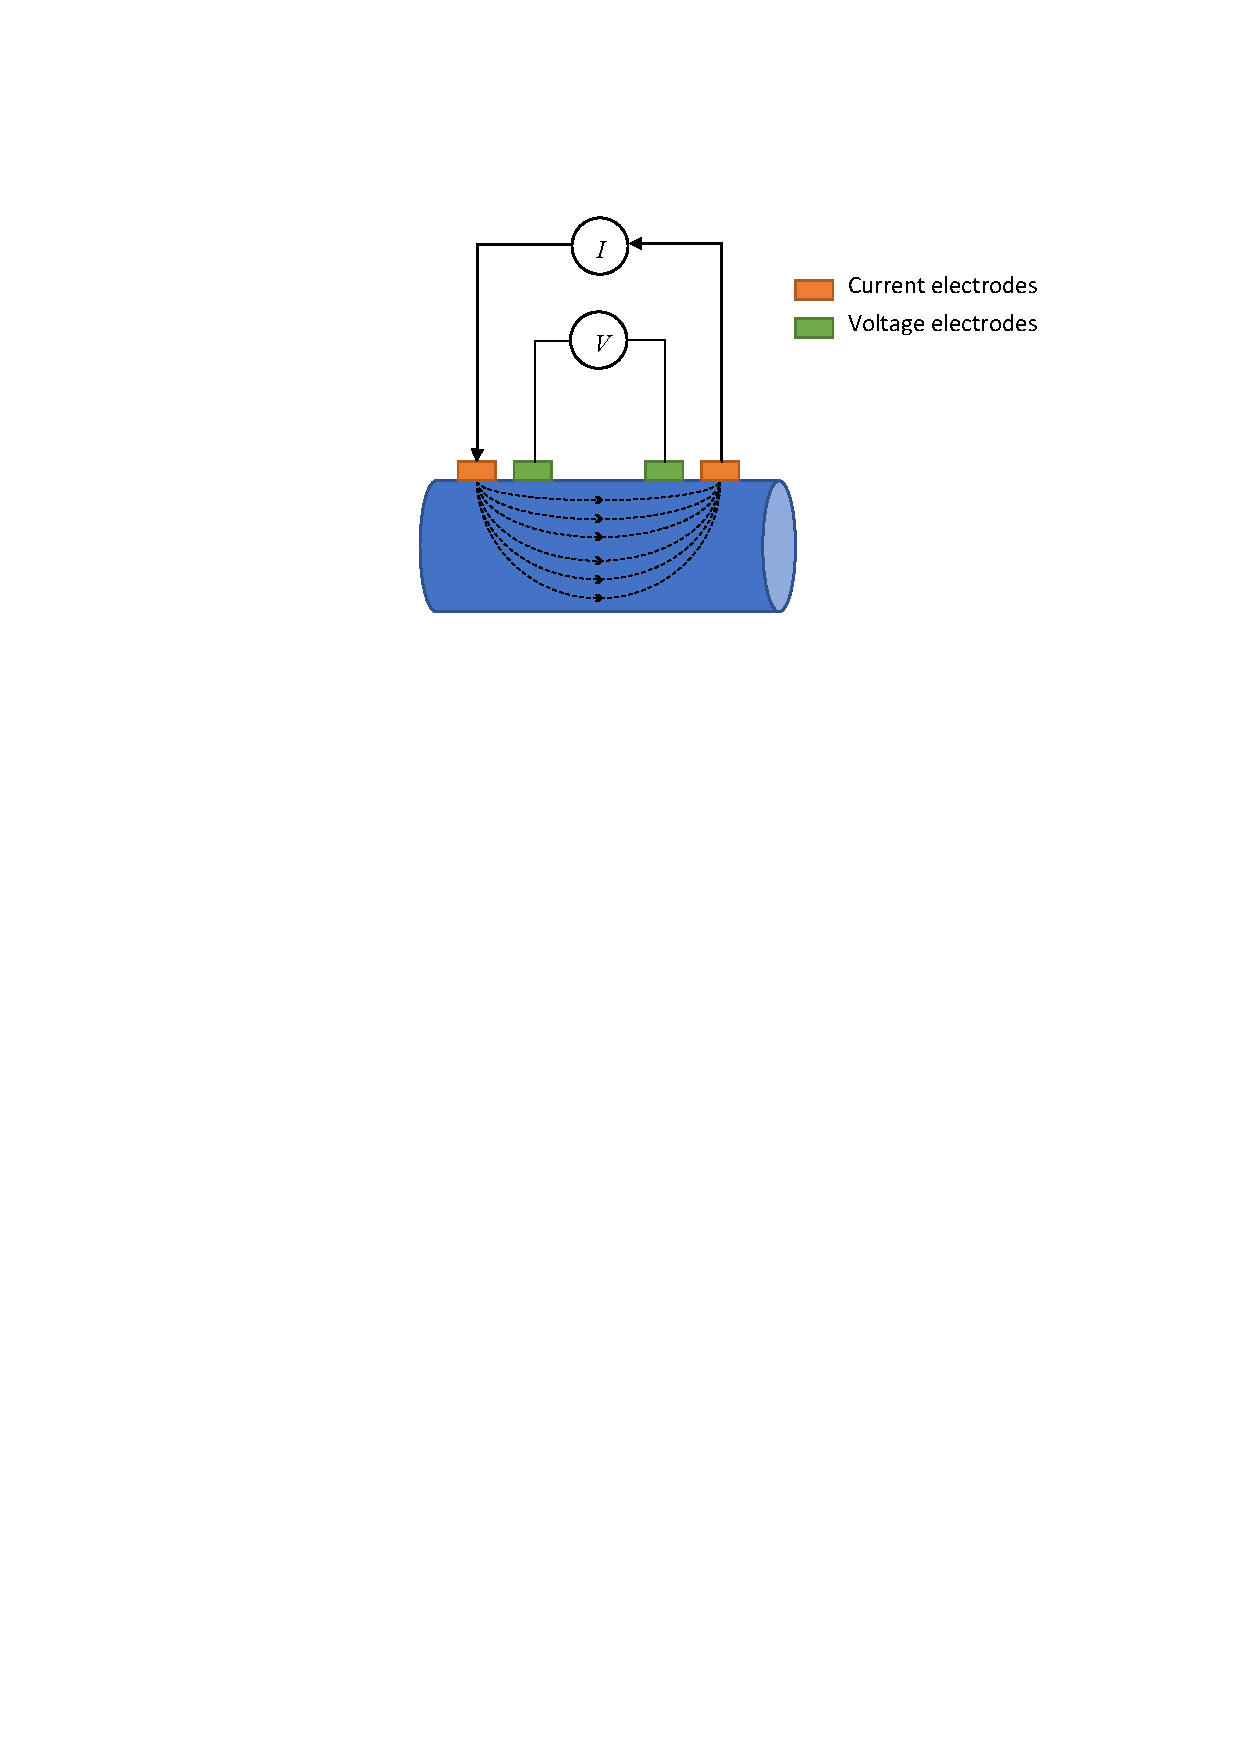
\includegraphics[width=0.5\textwidth,keepaspectratio]{tetrapolar_impedance}    
	\caption[Electrodes position in tetrapolar configuration]{Electrodes position in tetrapolar configuration. Outermost electrodes (current) inject current into the tissue. Inner electrodes sense the voltage drop caused by the tissue.}
	\label{fig:tetrapolar iPG}
\end{figure}

Another difference is the frequency used in iPG to measure impedance plethysmography; this usually ranges from \SIrange{10}{100}{\kilo\hertz} \cite{songer2001tissue,casas1999vivo,kun1994tissue,ristic1997muscle}. This level of frequency is large enough to avoid any muscle stimulation that could be hazardous for the patient. 

The electrical currents incorporated by this method are in the range of few micro-amperes (\si{\micro\ampere}) to few milliamperes (\si{\milli\ampere}), confining it within the limits of patient safety, as described in section \ref{section impedance current in body}. Clearly, the higher the current, the higher the voltage output response, as per Ohm's law ($v = R \times i$); this is because the body segment behaves like a resistor. To ensure patient safety, it is recommended that current is injected instead of voltage because circuits can limit the amount of injected electrical current and provide a better control on the amplitude of the waveform. Overall, the amount of current required to obtain a clean signal depends on the geometry of the volume being tested, the electrodes geometry, and the physiological attributes of the tissue. 

The data presented by an impedance device can be exhibited as a real or imaginary part of the impedance. However, it has been demonstrated that operating at these frequencies does not cause a major difference between the real part and the modulus of the measurement. In fact, the imaginary component of the signal is less than \SI{12}{\degree} \cite{jaffrin1979quantitative}. Therefore, the modulus of an impedance plethysmography measure provides sufficient information about the volume change in a limb section \cite{anderson1984impedance}. However, this phase might assume significance if higher frequencies are used to isolate a particular tissue or physiological event.

\begin{figure}[!htpb]
	\centering
	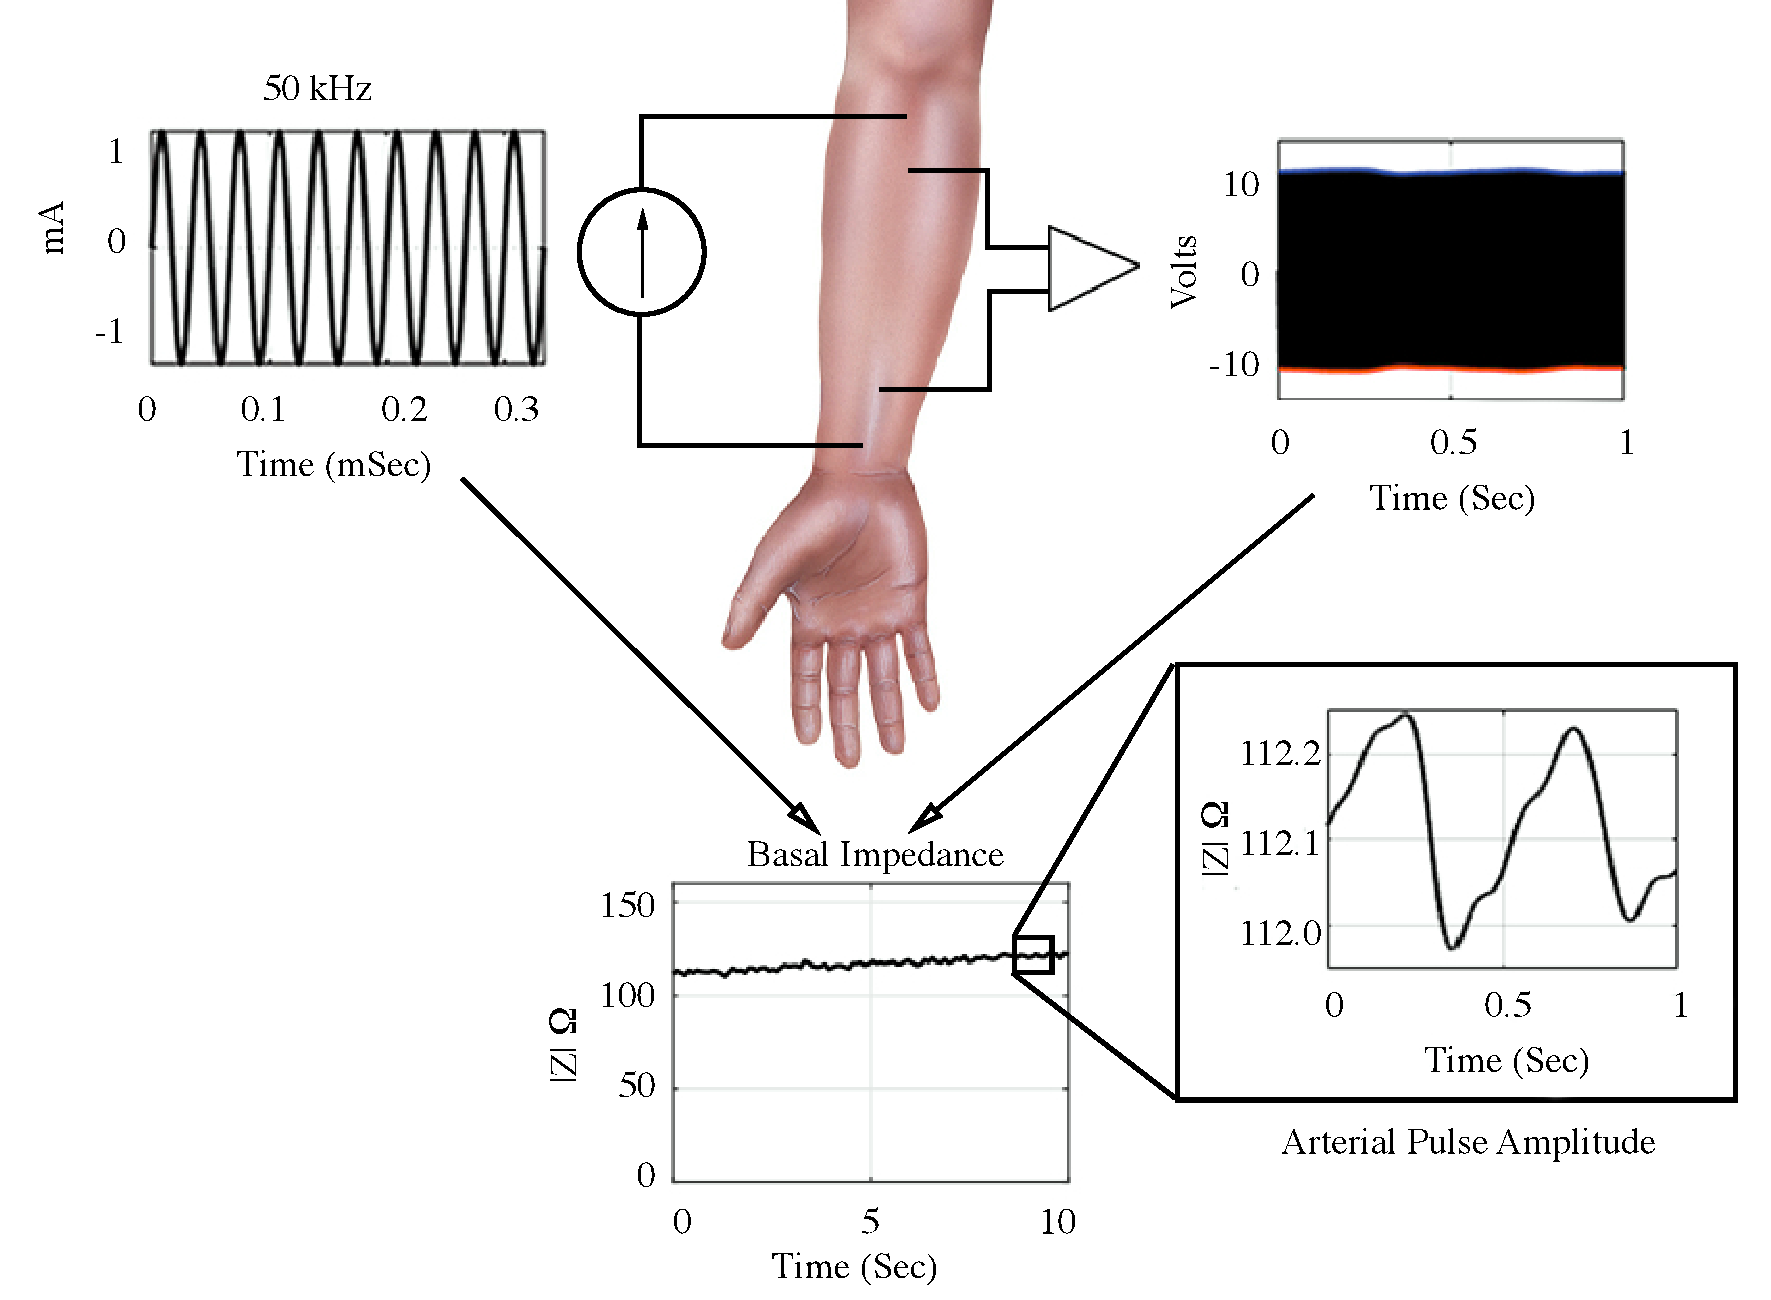
\includegraphics[width=\textwidth,keepaspectratio]{figure15}    
	\caption[How to get an impedance plethysmography waveform]{An impedance plethysmography waveform ban be obtained by applying a constant current and sensing the resultant voltage. The division between the potential and the current provides the impedance module - which is the basal impedance. The arterial pulse amplitude can be seen within the basal impedance.}
	\label{fig:envelope iPG}
\end{figure}

As illustrated by the figure \ref{fig:envelope iPG}, it is possible to obtain an impedance plethysmography signal by injecting the required current into the tissue at a specific frequency. One of the most common signals is \SI{50}{\kilo\hertz}. Once the electrical signals pass into the electrodes, they get transformed into an ionic conduction. The interaction of current with the tissue leads to a decline in voltage that can be detected by the sensing electrodes. From the electrical viewpoint, an amplitude modulated voltage waveform is generated from the tissue. However, this modulation remains synchronous to the heart cycle only represents \SI{0.1}{\percent} of the waveform \cite{anderson1984impedance}. 
The impedance modulus is obtained using Ohm's law (equation \ref{eq:|Z|}). The resultant impedance is known as either basal impedance (BI) or resting baseline impedance (RBI). Moreover, the underlying dynamic signal is known as arterial pulse amplitude (APA). 

\begin{align}
	\label{eq:|Z|}
	\left| Z \right| = \frac{v}{i}
\end{align}


\subsection{Blood contribution to impedance} %Section - 3.2.1
As mentioned before, impedance plethysmography depends on the volume change caused by blood vessels filling up all areas along the cardiac cycle; blood is highly conductive and influences the amplitude of the waveform. However, other particular properties might modify its intrinsic signal. In one of the earliest research works on the conductivity of blood, Sigman et al.~\cite{sigman1937effect} demonstrated that blood's resistivity depends on its flow. It was found that when blood velocity decreased from \SIrange{10}{40}{\centi\meter\per\second} its resistivity fell by roughly \SI{7}{\percent}. Furthermore, it was found that haematocrit and temperature also affect the blood resistivity \cite{yamakoshi1980noninvasive}. However, the temperature remains nearly constant in an in-vivo setting. Blood can be simplified as a suspension of particles (erythrocytes or RDC) using a high resistivity floating within a conductive medium (plasma). The remaining blood cells do not represent a significant component of the change of impedance owing to its small size in comparison with the erythrocytes (see table \ref{table:cell}). In fact, the Sigman effect is absent in either plasma or electrolytes~\cite{tremper1990principles}.  

Blood has also been proven to be electrically anisotropic due to the orientation of the RBC's \cite{Visser1992Electric}. Moreover, geometry and orientation also end up affecting the reading of resistivity, which means that direction of measurement also affects the readings. 

\subsection{Impedance plethysmography waveforms}
\label{section iPG waveforms}
The impedance plethysmography provides important information about the venous and arterial circulatory properties within a particular bodily segment. The impedance waveform comprises of a constant impedance value (basal impedance) and a dynamic component within it (arterial pulse amplitude). However, it is possible to obtain details about peripheral venous circulation when occluding a limb proximally. This kind of method is known as venous occlusion plethysmography (VOP).

\begin{figure}[!htpb]
	\centering
	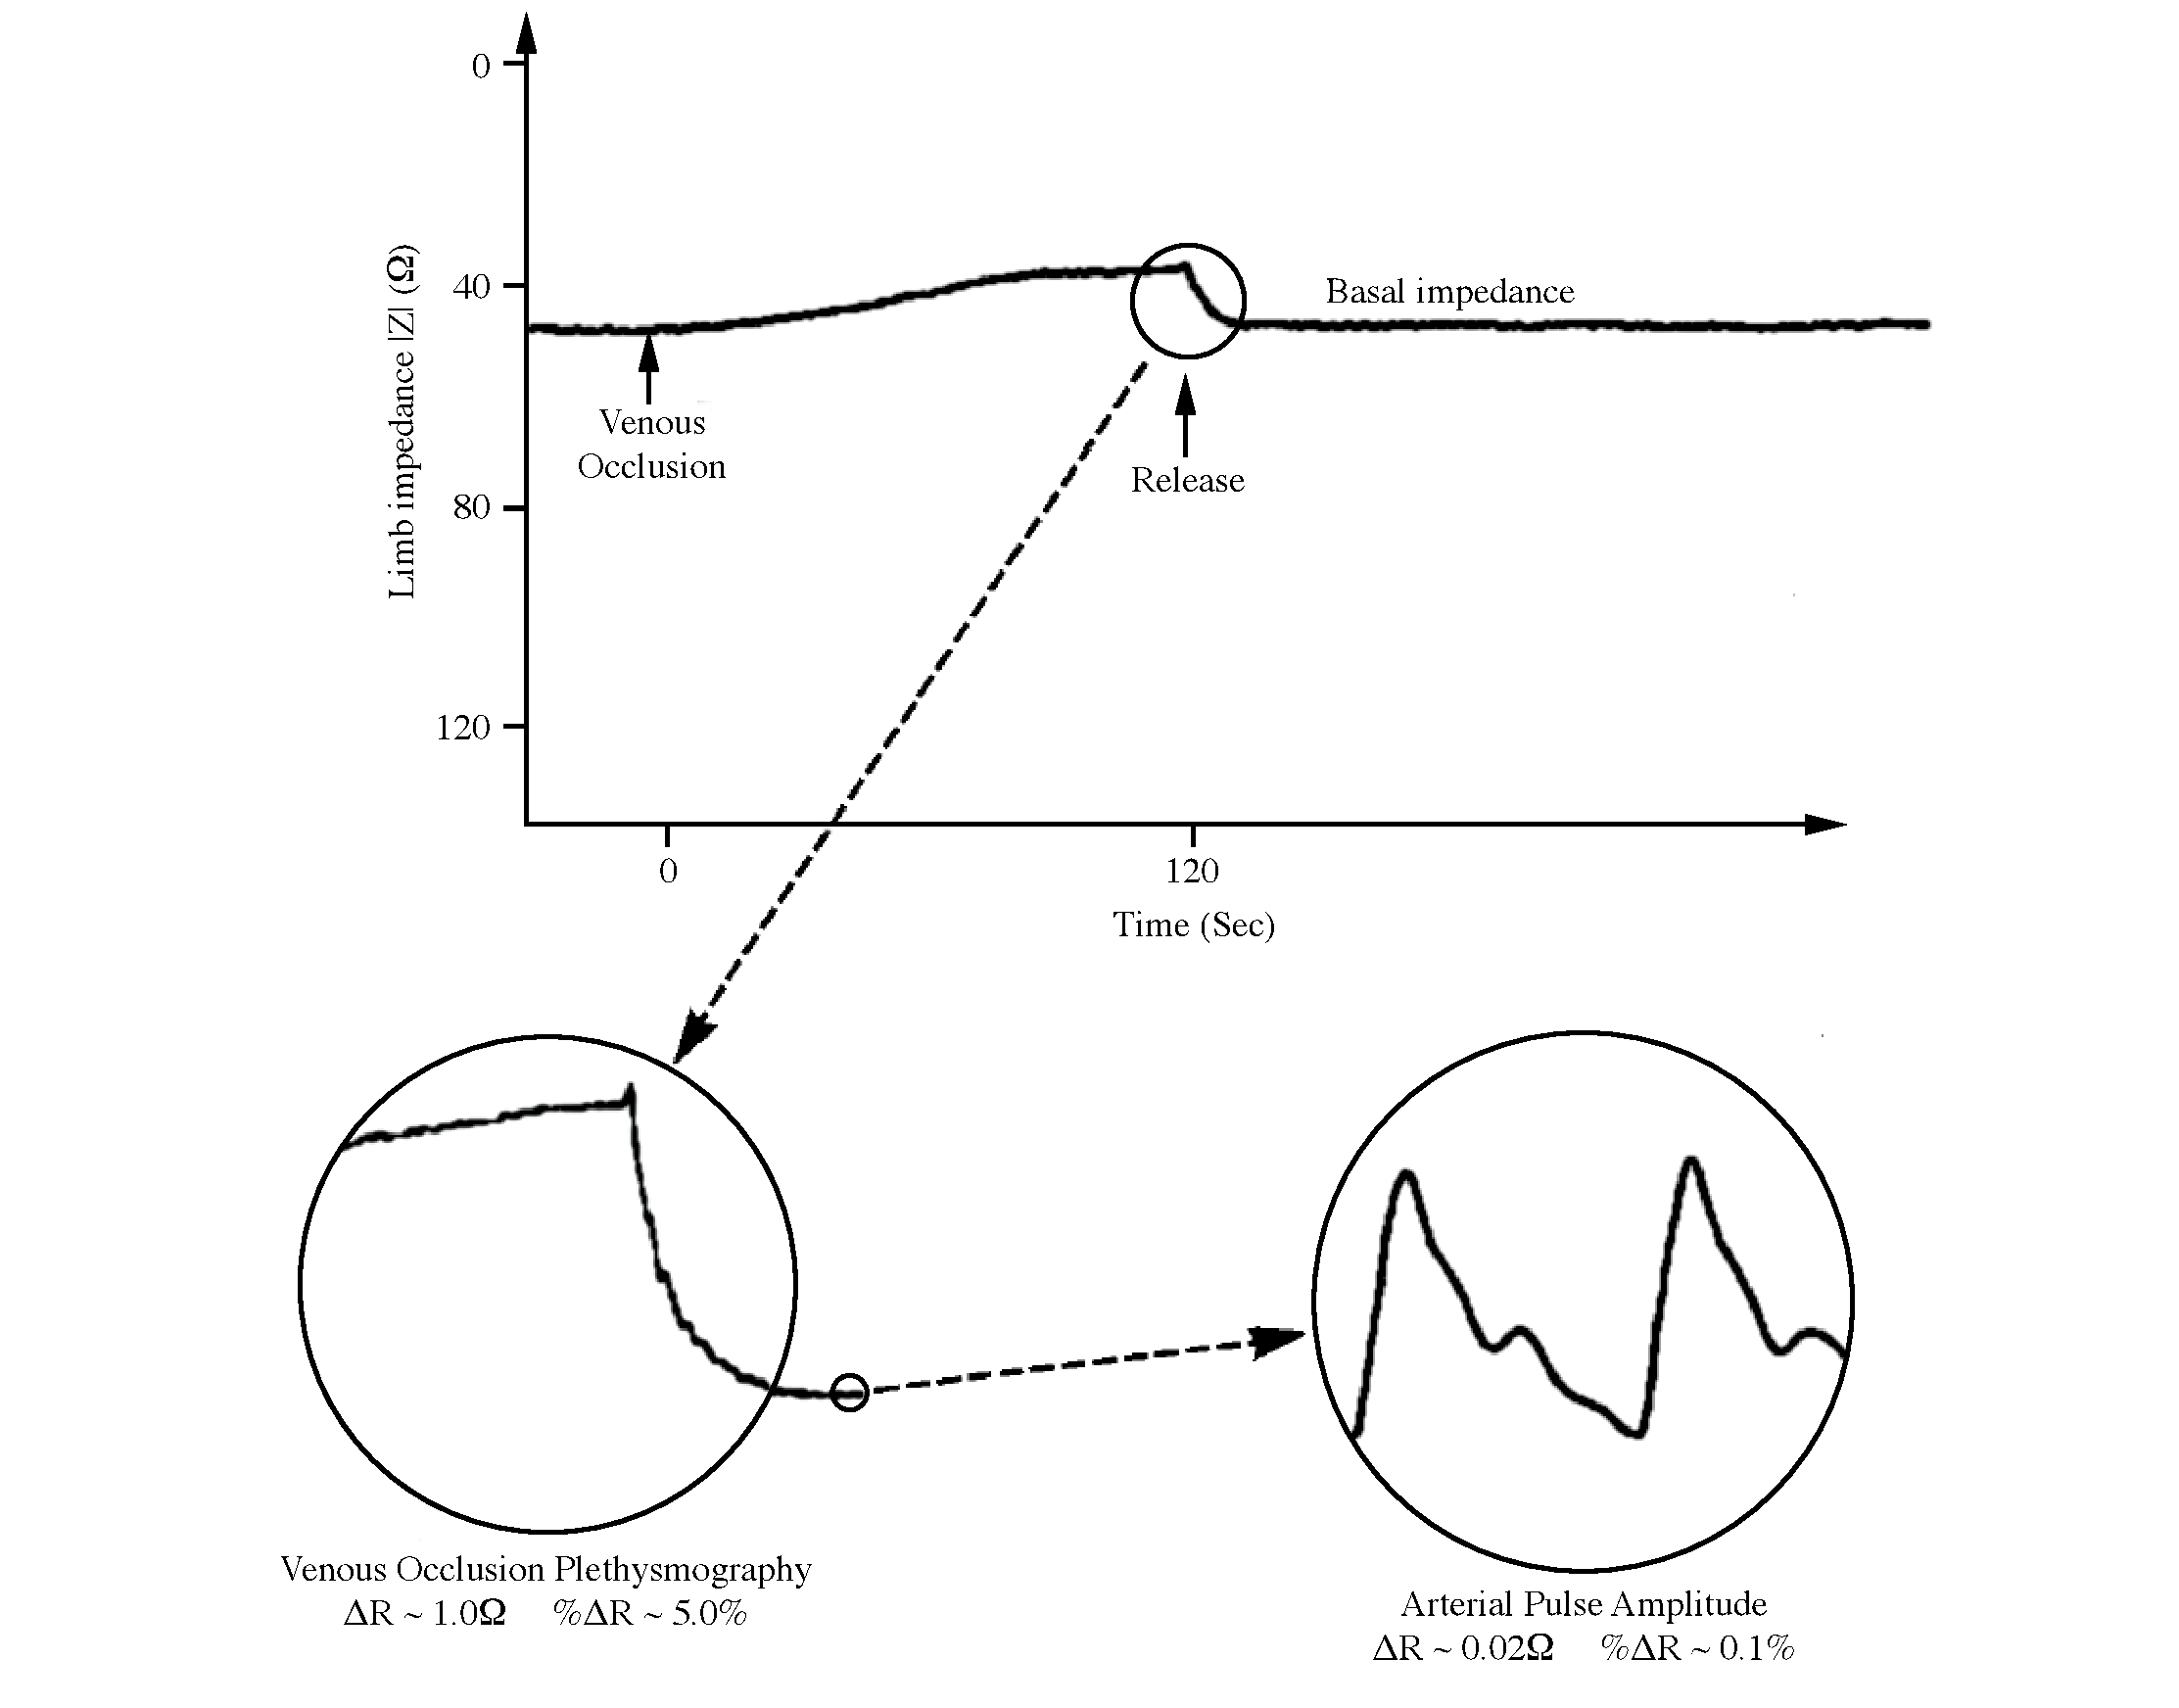
\includegraphics[width=\textwidth,keepaspectratio]{figure16}    
	\caption[Signal from an impedance plethysmography device]{An impedance plethysmography device can produce three signals: 1) the basal impedance or resting baseline resistance; 2) by using a blocking venous return at (\SIrange{40}{50}{\mmHg}) to extract the venous occlusion plethysmography wave; and 3) within the basal impedance is located the arterial pulse amplitude which changes with the heart beat. Adapted from \cite{anderson1984impedance}}
	\label{fig:iPG signals}
\end{figure}

Figure \ref{fig:iPG signals} shows the three different components of an impedance plethysmography waveform. The signal consists of the following components: basal impedance or resting baseline impedance (RBI), venous volumes changes and arterial pulses. 

\subsubsection{Basal impedance}
Also known as the resistive baseline impedance, this is the most significant data obtained from an impedance plethysmography device (see figure \ref{fig:iPG signals}). The main contributors to this impedance include muscles, blood and bones. The resistivity of muscles is about \SIrange{200}{300}{\ohm\cm}, whereas the resistivity of bone and fat is greater than \SI{2000}{\ohm\cm} and the blood resistivity is about \SI{150}{\ohm\cm} \cite{gabriel1996dielectric}. Therefore, this combination of impedances can be expressed as a parallel model of resistances wherein muscle and blood are the main contributors of the RBI. The range of this impedance value is from \SIrange{10}{100}{\ohm}. 

It has been demonstrated that it is possible to gather information about the development of ischemic tissue by studying the changes of baseline during a time. Some studies have shown that the impedance value increases during ischemic events in the bandwidth of \SIrange{1}{100}{\kilo\hertz} within different kinds of tissue \cite{songer2001tissue,casas1999vivo,kun1994tissue,ristic1997muscle} which is within the frequency measurement of iPG. 

\subsubsection{Venous occlusion plethysmography}
The second signal obtained from the baseline signal provides information about the venous volume changes. Variations in venous volume tone occur naturally during respiration, which causes a modulation of the signal during the respiratory cycle between \SIrange{0.2}{0.3}{\hertz}. However, by occluding the venous return, it is possible to produce larger volume variations represented as a greater displacement of the basal impedance of nearly\SI{1}{\Omega} or \SI{5}{\percent} from the mean value. 

The most common method to evaluate venous volume is known as venous occlusion plethysmography, which is quite common in the assessment of peripheral vascular diseases such as deep venous thrombosis. Impedance plethysmography VOP (see figure \ref{fig:iPG signals}) provides similar results as other well-established methods such as strain gauge\cite{schraibman1975comparison} and air/water displacement techniques \cite{fleming1986comparison}. This method requires occluding the limb's proximal section using a cuff with a pressure above the venous pressure staying usually about \SI{40}{\mmHg}.  The retention of the blood increases the volume of the limb with each heart cycle. The accumulation of blood in the measured segment increases its conductivity and reduces the total resistivity.  A deviation from up to \SI{10}{\percent} from the basal impedance can be achieved depending on the occlusive pressure, arterial inflow, venous tone, central venous pressure (CVP), and the capacity of the venous vascular bed. 

\subsubsection{Arterial pulse amplitude}
The third signal component of an impedance plethysmography is the arterial pulsations, which are waveforms synchronous with the heart cycle (\SIrange{1}{2}{\hertz}). This signal is just a fraction of the total impedance; it is just \SI{0.1}{\percent} of the total impedance signal - approximately \SI{0.02}{\ohm} in the limbs of healthy young adults. Obtaining this signal can be challenging since its values are in close proximity to noise levels. Therefore, the signal should be isolated by using sharp filters and averaging some pulses. Changes in  the waveform shape are attributed to different reasons such as tissue volume, arterial inflow, arterial vessel compliance, proximal occlusion, peripheral resistance as well as electrodes topology, geometry and location.  Changes in the signal amplitude are an indicator of arterial problems. For instance, arteriosclerosis reduces the arteries elasticity with age. Hence the arterial pulse amplitude reduces in magnitude.

\section{Conclusion}
Electrical impedance is the response that any conductive medium presents to an alternating current or voltage. It is frequency dependent and can be described as resistive ($R$) or reactive ($X$), which is determined by the resultant signal being in phase with the source or not. When applied to the human body, it is known as bioelectrical impedance, which is a non-invasive method that allows for the analysis of change in the human body using harmless and imperceptible AC. The current applied on any part of the body should be within the limits of patient safety. According to the literature, any current  lower than \SI{5}{\mA} is a good option but is also frequency dependent. 

Electrical impedance applied to humans can examine the health of tissue as well as changes in blood volume. The measurements produced by this method are attributed to the ions transport in tissue when a set of electrodes converts electrical current into ionic conduction. Bioelectrical impedance measurements can perform both whole body measurements and local body segments. It can be applied using either single or multiple frequencies, or to perform analysis over a wide range of the spectrum. 

Bioelectrical impedance plethysmography measures blood-related changes in the human body. It is commonly used in a tetrapolar configuration where a pair of electrodes injects current and a second couple measures the voltage drop. Instruments utilising this technology produce two types of data: \textit{basal impedance} is the whole impedance contribution of bones, muscle, fatty tissue, skin and blood. Under normal conditions, this signal tends to be unchangeable. However, within it lies another small signal that contains information about the arterial pulsations, known as \textit{arterial pulse amplitude}.


%********************************** %Nomenclatures in chapter  **************************************
\nomenclature[z-EM]{EM}{Electromagnetic}
\nomenclature[z-EIS]{EIS}{Electrical impedance spectroscopy}
\nomenclature[z-BLM]{BLM}{Bilayer lipid membrane}
\nomenclature[z-DLC]{DLC}{Dual layer capacitance}
\nomenclature[z-GSR]{GSR}{Galvanic impedance response}
\nomenclature[z-EWC]{EWC}{Extracellular water content}
\nomenclature[z-IWC]{IWC}{Intracellular water content}
\nomenclature[z-ICG]{ICG}{Impedance cardiography}
\nomenclature[z-PVT]{PVT}{Proximal vein thrombosis}
\nomenclature[z-BMI]{BMI}{Body mass index}
\nomenclature[z-BIVA]{BIVA}{Bioelectrical impedance vector analysis}
\nomenclature[z-SVR]{SVR}{Systemic vascular resistance}
\nomenclature[z-DSP]{DSP}{Digital signal processors}
\nomenclature[z-FFM]{FFM}{Free-fat mass}
\nomenclature[z-TBW]{TBW}{Total body water}
\nomenclature[z-ALS]{ALS}{Amyotrophic lateral sclerosis}
\nomenclature[z-BCM]{BCM}{Body cell mass}
\nomenclature[z-IEC]{IEC}{International Electrotechnical Commission}
\nomenclature[z-VF]{VF}{Ventricular fibrillation}
\nomenclature[z-RF]{RF}{Radio frequency}
\nomenclature[z-RMS]{RMS}{Root mean square}
\nomenclature[z-BI]{BI}{Basal impedance}
\nomenclature[z-RBI]{RBI}{Resting baseline impedance}
\nomenclature[z-APA]{APA}{Arterial pulse amplitude}
\nomenclature[z-VOP]{VOP}{Venous occlusion plethysmography}
\nomenclature[z-CVP]{CVP}{Central venous pressure}
\nomenclature[z-GSR]{GSR}{Galvanic impedance response}
\nomenclature[z-BIA]{BIA}{Bioelectrical impedance analysis}